%%%%%%%%%%%%%%%%%%%%%%%%%%%%%%%%%%%%%%%%%%%%%%%%%%%%%%%%%%%%%%%%%%%%
%% I, the copyright holder of this work, release this work into the
%% public domain. This applies worldwide. In some countries this may
%% not be legally possible; if so: I grant anyone the right to use
%% this work for any purpose, without any conditions, unless such
%% conditions are required by law.
%%%%%%%%%%%%%%%%%%%%%%%%%%%%%%%%%%%%%%%%%%%%%%%%%%%%%%%%%%%%%%%%%%%%

\documentclass[
  digital, %% The `digital` option enables the default options for the
           %% digital version of a document. Replace with `printed`
           %% to enable the default options for the printed version
           %% of a document.
%%  color,   %% Uncomment these lines (by removing the %% at the
%%           %% beginning) to use color in the printed version of your
%%           %% document
  oneside, %% The `oneside` option enables one-sided typesetting,
           %% which is preferred if you are only going to submit a
           %% digital version of your thesis. Replace with `twoside`
           %% for double-sided typesetting if you are planning to
           %% also print your thesis. For double-sided typesetting,
           %% use at least 120 g/m² paper to prevent show-through.
  lof,     %% The `lof` option prints the List of Figures. Replace
           %% with `nolof` to hide the List of Figures.
  lot,     %% The `lot` option prints the List of Tables. Replace
           %% with `nolot` to hide the List of Tables.
]{fithesis4}
%% The following section sets up the locales used in the thesis.
\usepackage[resetfonts]{cmap} %% We need to load the T2A font encoding
% \usepackage[T1,T2A]{fontenc}  %% to use the Cyrillic fonts with Russian texts.
\usepackage[
  main=english, %% By using `czech` or `slovak` as the main locale
                %% instead of `english`, you can typeset the thesis
                %% in either Czech or Slovak, respectively.
  english, czech %% The additional keys allow
]{babel}        %% foreign texts to be typeset as follows:
% \usepackage[utf8x]{inputenc}
\usepackage[utf8]{inputenc}

\inputencoding{utf8}
\DeclareUnicodeCharacter{0301}{\'{e}}
% \usepackage[cp858]{inputenx}
% \DeclareUnicodeCharacter{0160}{\v{S}}
% \DeclareUnicodeCharacter{04F1}{\"\cyru}
% \DeclareUnicodeCharacter{04F2}{\H\CYRU}
% \DeclareUnicodeCharacter{04F3}{\H\cyru}
% \usepackage{newunicodechar}
% \newunicodechar{�}{x}
% Šumperk
\usepackage{textcomp}

%% For non-Latin scripts, it may be necessary to load additional
%% fonts:
\usepackage{paratype}
% \def\textrussian#1{{\usefont{T2A}{PTSerif-TLF}{m}{rm}#1}}
%%
%% The following section sets up the metadata of the thesis.
\thesissetup{
    date        = \the\year/\the\month/\the\day,
    university  = mu,
    faculty     = fi,
    type        = mgr,
    department  = Department of Machine Learning and Data Processing,
    author      = {Ing. Štěpán Skovajsa},
    gender      = m,
    advisor     = {RNDr. Petr Novotný, Ph.D.},
    title       = {Modelling of Infection Risk via Probabilistic Programming},
    keywords    = {Bayes theorem, Bayesian inference, Probabilistic programming, Probabilistic modelling, PyMC3, Monte-Carlo simulation, Covid-19, Epidemiology, Infection risk, Disease, SIR model, Reproduction number},
    abstract    = {%
In epidemiology, there is no holy grail for modelling the risk of infection.
Usually, the epidemiologists publish reports with daily incidence and reproduction numbers as a product of some epidemiological model. Unfortunately, common people find reproduction numbers less interpretable, and incidence does not reveal much risk information. Moreover, in most cases, these estimates of the reproduction numbers are approximated for broader geographical segments as whole states and usually not for smaller areas such as regions or districts.

This thesis provides a basic epidemiological theory to understand modelling of infection spread. Later, it utilizes that theory to build a robust solution to estimate the risk of infectious contact, based only on the daily incidence. This solution is divided into two parts: the incidence model, where the MCMC with Gaussian process smoothens incidence observations, and the risk model, in which we use the estimated incidence to obtain the risk of infectious contact. This solution can work with very noisy and zero-inflated data.

The results found that the solution approaches the risk well on synthetically generated data. According to the real-world data, the solution underestimates the prevalence, hence underestimates the risk. Therefore it requires far more tuning to be more practical.
    },
    thanks      = {%
I would like to thank my supervisor, RNDr. Petr Novotný,~Ph.D.,~especially for introducing me to probabilistic modeling and the challenge I was able to take by choosing this thesis proposal. Also, for his guidance, support, and valuable advices, he provided for the entire process. I would also like to thank every author of each title mentioned in the bibliography for their work, so I was able to build this thesis. Furthermore, I will not forget to thank my family and girlfriend for their endless support.
    },
    bib         = references.bib,
    %% Remove the following line to use the JVS 2018 faculty logo.
    facultyLogo = fithesis-fi,
}
\usepackage{makeidx}      %% The `makeidx` package contains
\makeindex                %% helper commands for index typesetting.
% \usepackage[acronym]{glossaries}          %% The `glossaries` package
% \renewcommand*\glspostdescription{\hfill} %% contains helper commands
% \loadglsentries{example-terms-abbrs.tex}  %% for typesetting glossaries
% \makenoidxglossaries                      %% and lists of abbreviations.
%% These additional packages are used within the document:
\usepackage{paralist} %% Compact list environments
\usepackage{amsmath}  %% Mathematics
\DeclareMathOperator*{\argmax}{arg\,max}
\DeclareMathOperator*{\argmin}{arg\,min}
\usepackage{amsthm}
\usepackage{amsfonts}
\usepackage{amssymb}
\usepackage{url}      %% Hyperlinks
\makeatletter
\g@addto@macro{\UrlBreaks}{\UrlOrds}
\makeatother
\usepackage{markdown} %% Lightweight markup
\usepackage{listings} %% Source code highlighting
\lstset{
  basicstyle      = \ttfamily,
  identifierstyle = \color{black},
  keywordstyle    = \color{blue},
  keywordstyle    = {[2]\color{cyan}},
  keywordstyle    = {[3]\color{olive}},
  stringstyle     = \color{teal},
  commentstyle    = \itshape\color{magenta},
  breaklines      = true,
}
\renewcommand{\lstlistingname}{Snippet}
\usepackage{floatrow} %% Putting captions above tables
\floatsetup[table]{capposition=top}
\usepackage[babel]{csquotes} %% Context-sensitive quotation marks
\begin{document}
%% Uncomment the following lines (by removing the %% at the beginning)
%% and to print out List of Abbreviations and/or Glossary in your
%% document. Titles for these tables can be changed by replacing the
%% titles `Abbreviations` and `Glossary`, respectively.
%% \clearpage
%% \printnoidxglossary[title={Abbreviations}, type=\acronymtype]
%% \printnoidxglossary[title={Glossary}]

%% The \chapter* command can be used to produce unnumbered chapters:
\chapter*{Introduction}
%% Unlike \chapter, \chapter* does not update the headings and does not
%% enter the chapter to the table of contents. I we want correct
%% headings and a table of contents entry, we must add them manually:
\markright{\textsc{Introduction}}
\addcontentsline{toc}{chapter}{Introduction}

Epidemiology subsumes several science disciplines like biology, math, social sciences.
The nature of an epidemic disease is the cause - it is invisible for our eyes but might have a significant impact on our health and society at all.
It may start with investigating a disease from a microbiological perspective in a laboratory, through disease tracking of infected people and sudden mathematical modelling, ending with government interventions like social distancing, healthcare crisis management, vaccination strategy, financial and other support for most affected segments or areas.

The previously mentioned mathematical modelling may be used in various perspectives for epidemiology. 
For example, it may be used to understand better how a disease is spread and the risk of being infectious or succumbing to disease.
From that medical perspective, mathematical modeling provides a foundation to prevent the spread of disease and minimalize health damage.
On the other hand, mathematical modelling can also be used to model socio-economical impact due to lockdowns, quarantine, and modelling business decisions during a pandemic.

For example, both perspectives can use medical and statistical data about a disease, demographic and socio-economic data about population, their transitivity between regions. 
Also, methods for finding solutions are quite similar. 
The main difference between those perspectives lies in the model, which is the mathematical formulation of a problem we want to solve. 
Unfortunately, it is pretty challenging to count all possible cases and situations, especially when there is not good enough data, so it is unrealistic to model diseases precisely. 
Instead, we make approximations of the natural world with the best data available with respect to a specified precision.

The basic reproduction number $\mathcal{R}_0$ and the effective reproduction number $\mathcal{R}_e$ are often parts of reports published by epidemiologists and other related experts.
For common people (i.e., non-epidemiologists), those indicators may be insufficient or incomprehensible in the basic sense.
Moreover, those indicators are usually reported for whole countries, not for lower administrative units such as cities, districts, or regions. 
For these reasons, this thesis presents more human-friendly probabilistic approach to the systematic epidemic risk of infectious contact.

The following section describes the probabilistic approach that is chosen in this work\footnote{Python notebook of this thesis is deployed at \url{https://colab.research.google.com/drive/1ld7uF0w3gILSaOnog7JkJXOo82V8JPeh?usp=sharing}}. 
However, several non-trivial questions will be arisen there, which will be gradually developed and answered in the following chapters to have a complete solution in the final stage.



\chapter{The risk as a probability}
\label{chap:risk-as-probability}

The risk itself can be, in very general taxonomy, seen from \textit{idiosyncratic} and \textit{systematic} perspective.
\textit{Systematic risk} is the more general one. It affects everyone, or at least, everyone in the substantial sample considerable as a population (e.g., citizens of a city, disease-susceptible seniors in a country).
On the contrary, the \textit{idiosyncratic risk} is the specific (individual) type of risk, which is more focused on a small sample of individuals.
An excellent example of idiosyncratic risk is superspreaders, the infected individuals with usually low frequency of occurrence, but with the ability to infect an excessive amount of people \cite[Chapter~4]{brauer2008}.
That makes idiosyncratic risk more difficult to grasp.
Therefore, we will focus on the systematic risk only.

In the quantitative risk assessment way of thinking, the risk can be perceived as a probability \cite[Chapter~14]{bahr2014}.
In our case, the risk we model will be a probability of infectious contact.
This mean we are looking for the probability of meeting at least one infected individual given the number of random contacts:

\begin{equation}\label{eq:risk-first}
  \text{risk} = P(\text{infectious contact} | \text{number of contacts})
\end{equation}

Let $N$ denote the size of a population and $I$ the number of infected individuals among that population, thus $I \leq N$.
Assuming the infectious $I$ are uniformly distributed across the population, then $p = \frac{I}{N}$ is the probability of selecting an infected individual.
This corresponds to the \textit{Bernoulli distribution} \cite{bernoulli-dist}:

\begin{equation}
  X \sim \text{Bernoulli} \left( p \right)
\end{equation}

where $X$ corresponds to the dichotomous random variable ($X = 1 \Rightarrow \text{infectious}$, $X = 0 \Rightarrow \text{non-infectious}$).

Now lets bring the \textit{number of contacts} from \eqref{eq:risk-first} into the computation.
This quantity can be imagined as the size of the sample of people the investigated individual (the one for whom we compute the risk) has met previously.
If we denote the size of this sample $n$, we are basically interested in the number of infected individuals $i$ in that sample such that $i \leq n$. We can rewrite \eqref{eq:risk-first} as:

\begin{equation}\label{eq:risk-second}
  P(i \geq 1 | n)
\end{equation}

As we assume $i$ to be a discrete random variable, the discrete probabilistic distributions should be considered.
Namingly \textit{binomial}, \textit{negative binomial} and \textit{hypergeometric} distributions.

Both the binomial and negative binomial distributions are built on top of independent Bernoulli trials.
That assumes the probability $p$ of selecting each particular individual is the same, which is theoretically not true for our case because we are basically taking samples without replacement.
This means the probability of choosing each individual changes during the sampling process, i.e., the sampled individual is no longer part of the remaining population to sample.
This is valid for the \textit{hypergeometric distribution} \cite{hypergeometric-dist}.
Therefore, the \textit{probability mass function} for $i$ given the $N$, $I$ and $n$ will be:

\begin{equation}
  p(i|n) = \frac{ \binom{I}{i} \binom{N - I}{n - i} }{ \binom{N}{n} }
\end{equation}

where $\binom{a}{b}$ is a binomial coefficient.
We assume the validity of the p.m.f. for the condition $max\left( 0, I - N + n \right) \leq i \leq min\left( I, n \right)$.
However, p.m.f. is a probability that exactly $i$ infected individuals occupy the sample.
For sure, we can use a cumulative distribution function to express the probability of $i$ or less.
Normally, we would do something like $1 - P(X \leq x)$ to obtain the probability of at least one infectious in the sample, but we can imagine the probability of one and more infected individuals as a complementary to the probability that no one is infected; therefore, the risk  probability may be assumed as:

\begin{equation}\label{eq:risk-theoretic}
  P(i \geq 1|n) = 1 - p(i=0|n) = 1 - \frac{
    \binom{N - I}{n}
  }{
    \binom{N}{n}
  }
\end{equation}

As the $N$ and $n$ are known values, and $i$ is the quantity the probability of which we want to know.
The remaining question is how to approach the value of $I$.

This thesis provides a probabilistic solution to the above problem, but before we dive in, we have to introduce epidemiological fundaments first because every data science project requires particular \textit{domain knowledge} to understand the problem deeply, and this is not an exception.


\chapter{Epidemiological prerequisites}
\label{chap:epidemiological-prerequisites}

This chapter provides a fundamental insight into the mathematical epidemiology, i.e., history of mathematical modelling to highlight gradual development of mathematical methods, basic terminology used both in epidemiology and this thesis, and the most basic mathematical models.
The following basic epidemiologic overview will help the reader to understand the whole concept of how the solution was built.

During the gradual development of history, the people registered several deadly diseases of unknown origin.
Then survivors tended to investigate the causes of those fatalities to avoid future outbreaks or mitigate their effects.
In that sense, the science about disease spread prevention has started to arise.
\textit{U.S. Department of Health and Human Services Centers for Disease Control and Prevention} (\textit{CDC}) provides the following definition for \textit{epidemiology} \cite{cdc2006}:

\begin{displayquote}
  ``Epidemiology is the study of the distribution and
  determinants of health-related states or events in specified
  populations, and the application of this study to the control
  of health problems.''
\end{displayquote}

Nowadays, mathematical modelling is a necessary step when a disease outbreak occurs, starting with the computation of $\mathcal{R}_0$ (more on this later) to reveal the severity of the disease.
Later, it helps with decision-making during the pandemic state, keeping the population safe according to health, social-economic criteria.


\section{History of mathematical modelling in epidemiology}

The first study of this type considered was the 1663 book by John Graunt addressing methods of public health statistics.
In 1766, Daniel Bernoulli analyzed smallpox in his work, considered the first epidemiological model.
Then, the biological aspects of viruses and diseases were studied primarily by leading scientists of the time, such as Louis Pasteur and Robert Koch.
The mathematical modelling contributions were made later in the early twentieth century \cite[Chapter~1.4]{martcheva2015}.
William Hamer\footnote{\url{https://history.rcplondon.ac.uk/inspiring-physicians/sir-william-heaton-hamer}} was the first to use the law of mass action to model the recurrence of measles. 
Sir Ronald Ross\footnote{\url{https://en.wikipedia.org/wiki/Ronald_Ross}} is considered the founder of modern mathematical epidemiology due to his contribution to the mathematical modelling of malaria transmission.
He derived a threshold quantity, which is nowadays known as a \textit{basic reproduction number} denoted by $\mathcal{R}_0$.
Unfortunately, the mathematical modelling of diseases was not very accepted by the professional community at his time.
The change of mind in this field was brought by the invention of mathematical foundations of compartment models (SIR model to be more specific) in 1927 by W. O. Kermack and A. G. McKendrick \cite{kermack1927}.



\section{Epidemiological glossary}

The picture in the Figure \ref{fig:epidemiologists-bathtub} explains the most basic terms such as \textit{incidence}, \textit{prevalence}, \textit{mortality} and \textit{recovery} in the bathtub analogy:

\begin{figure}[h]
  \begin{center}
    
\includegraphics[width=8cm]{static/images/epidemiologists-bathtub.png}
  \end{center}
  \caption{The bathtub analogy \cite{steward2020}}
  \label{fig:epidemiologists-bathtub}
\end{figure}

Let the bath represent a set of infectious individuals at a certain time.
The size of this set is so-called \textit{prevalence} (sometimes also referred as \textit{active cases} number) for that time.
The prevalence can be \textit{increased} or \textit{decreased} when time is shifted forward.
The increase is referred to as the \textit{incidence} (will be mostly denoted $c$ here).
The decrease of prevalence may be done in two ways:
the infected individual dies - increase in \textit{mortality}, or, the infected individual gets restored from the disease - \textit{recovery} increase.
If we do not distinguish the way of decrease, we say that the individual was \textit{removed}.

Basically, from the perspective of a specific case, the disease is transmitted between \textit{infector} $A$ and \textit{infectee} $B$.
The \textit{infector} (also known as a \textit{primary case}) is the one who carries the disease and \textit{infectee} (also known as a \textit{secondary case}) is the susceptible person, which is being infected.
We also study \textit{infection age} (denoted $a$ here), which is the time for how long the specific individual is infected.
If the infector $A$ infects infectee $B$, it is done at infector's infection age $a_A > 0$, and when the transmission of infection succeeds, the infectee starts its own infection age $a_B = 0$.
This abstraction allows specifying several essential time intervals.

\begin{figure}[H]
  \begin{center}
    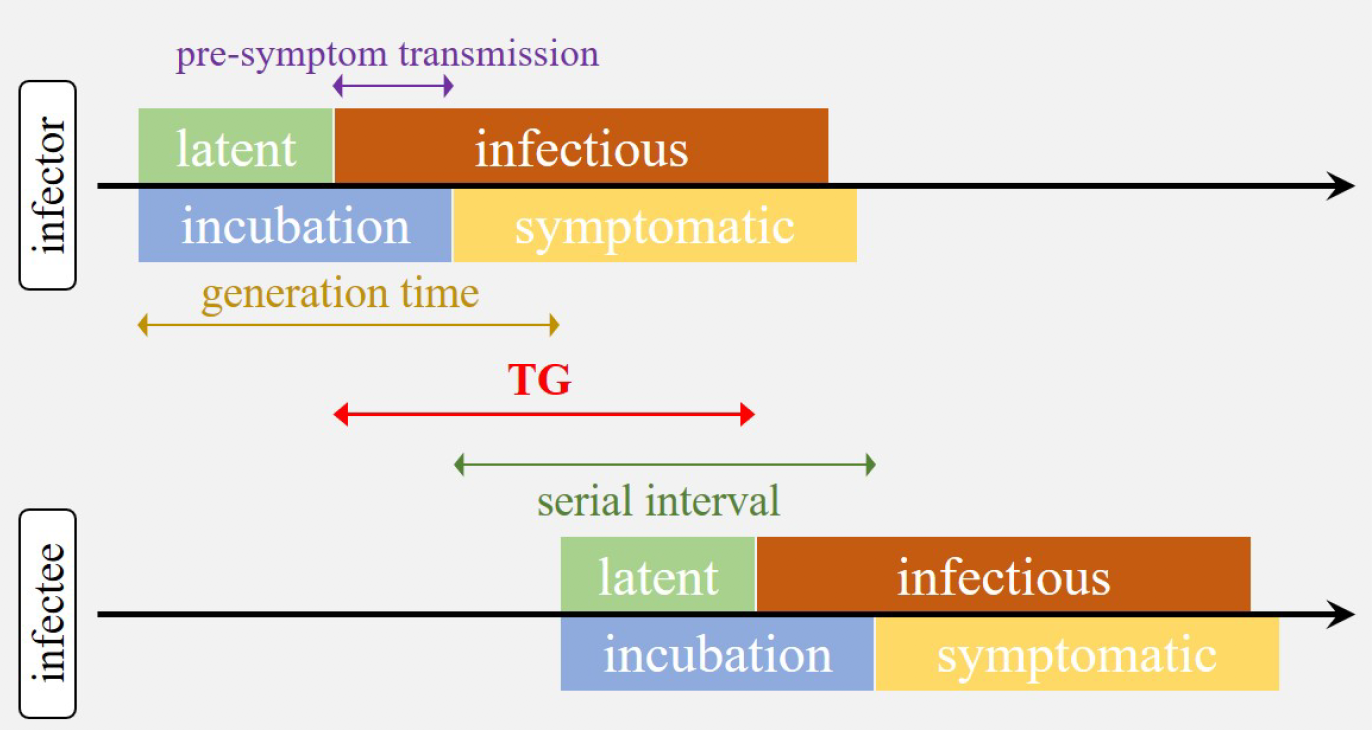
\includegraphics[width=11cm]{static/images/zhao2020_terms.png}
  \end{center}
  \caption{The demonstrative timeline of a transmission chain for a pair of infector and infectee \cite{zhao2020}}
  \label{fig:zhao-transmissive-chain-example}
\end{figure}

The most important time intervals are 
the \textit{incubation period} $h$, \textit{serial interval} $s$ and \textit{generation time} $g$.
\textit{Incubation period} is the time between exposure up to the time of symptoms onset.
In this period, the infected is usually not aware about his infection.
It is revealed later when the \textit{symptomatic period} begins.
\textit{Generation time} is the exact time period between the time the infector was infected and the time the infector infected the infectee.
The \textit{serial interval} has similar nature.
It is the time period between the onset symptoms in the infector and the onset of symptoms noticed on the associated infectee.

When the infector infects the infectee before the infector's
symptoms appear, we call it \textit{presymptomatic transmission}, i.e.,
the infectee was infected in the infector's \textit{incubation period}
(as shown in the Figure \ref{fig:nishiura-transmission}).

When $s < 0$, the infectee's symptoms occurred earlier than the infector's.
On the other hand, $g > 0$ is always
valid because the infector is always infected earlier than the infectee.

\begin{figure}[h]
  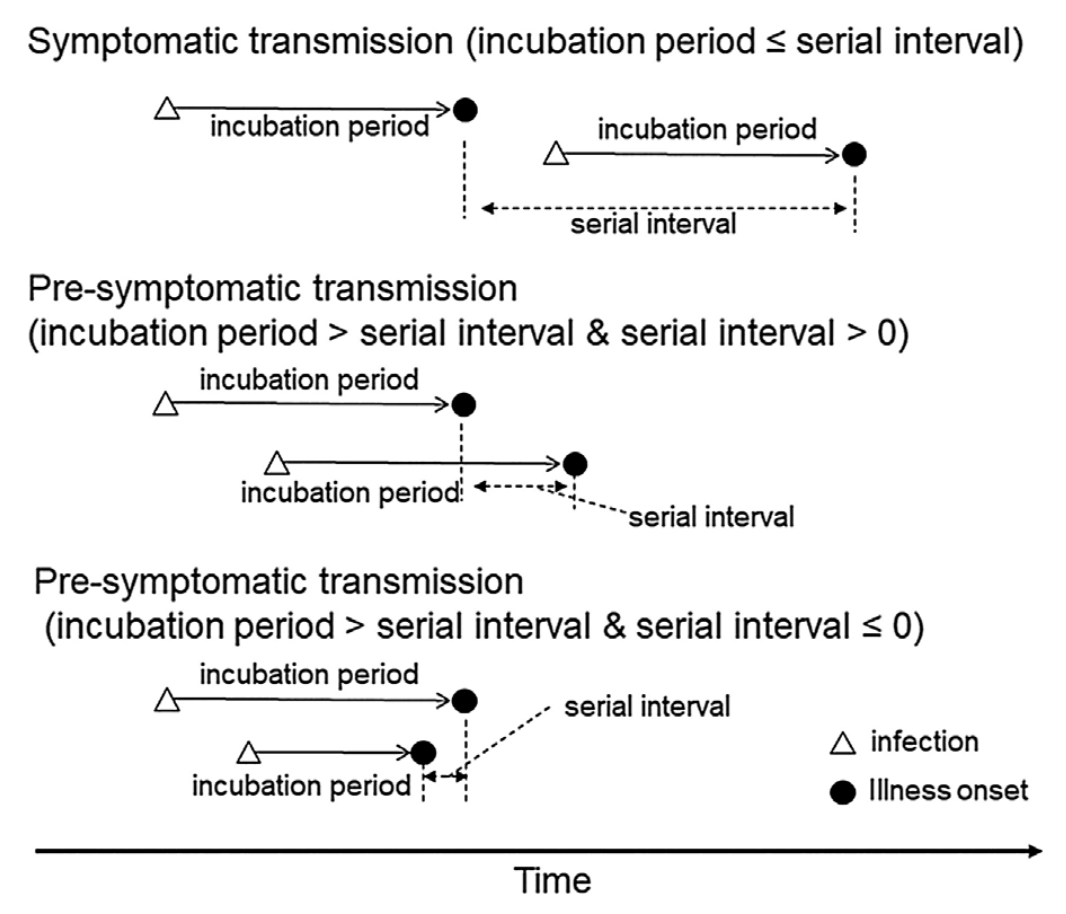
\includegraphics[width=10cm]{static/images/nishiura2020_terms.png}
  \caption{The relationship between the incubation period and serial interval. \cite{nishiura2020}}
  \label{fig:nishiura-transmission}
\end{figure}


\section{Kermack–McKendrick model}

The first well-known model (generally 
known as \textit{SIR model}), proposed in 1927 by 
William Ogilvy Kermack and Anderson Gray McKendrick, and is 
usually used as an introductory model to the epidemic 
modeling \cite{martcheva2015} due to its simplicity, and
often serves as a foundation for more complex 
models (\cite{clancy2008} for example).

The SIR model divides entire population into three disjunct 
sets, called \textit{classes} or \textit{compartments} (hence the general 
name \textit{compartment models} \cite{bacaer2011}):

\begin{itemize}
  \item \textit{Susceptibles (size denoted $S$)} - a set containing non-infected individuals, but with the possibility to become infected.
  \item \textit{Infectious (size denoted $I$)} - individuals who are infected and also able to infect susceptible individuals.
  \item \textit{Recovery / Removed (size denoted $R$)} - those who were restored from the illness (and gained immunity) or those who died. In both cases, they are removed from susceptibles and infectious sets, and therefore, they do not play any further role.
\end{itemize}

To define the SIR model, let us explain the \textit{force of infection} first.
The force of infection, noted $\lambda$, is similar to potential energy in physics. In this case, it expresses 
the potential spreading force of the infectious compartment:

\begin{equation}
	\lambda = \tau \rho I,
\end{equation}

\noindent
where $\rho$ is the average contact rate of a person within the whole population, no matter if they are susceptible, infectious or removed.
Let $N$ be the size of the population, then $\rho N$ is the \textit{average number of contacts}.
Assuming the susceptibles are independently and identically distributed, the probability of selecting any susceptible in the population is equal to $\frac{S}{N}$.
Therefore $\rho N\frac{S}{N}$ is the number of contacts each infected individual makes with susceptibles (simplifies to $\rho S$).
$\tau$ is the probability of becoming infectious for susceptible who has met an infected individual:

\begin{equation}
	\tau = p \left( B~\textrm{is infected from}~A~|~B~\textrm{has contact with}~A \right)
\end{equation}

If the previous equations are combined together, $\tau \rho S$ can be assumed as the number of susceptibles who became infectious after they have met one infected individual per unit of time.
Now the incidence may be formulated as:

\begin{equation}
	c = \tau \rho I \frac{S}{N} = \lambda \frac{S}{N}
\end{equation}

One typically denotes $\tau \rho$ as $\beta$ and substitutes it into previous equation to get:

\begin{equation}
	c = \beta I \frac{S}{N}
\end{equation}

The compartment models are usually specified as a set of differential equations.
Let us start with the compartment of the susceptibles $S$. In the basic SIR model, the $S$ can be decreased only (as it assumes that everyone can be infected only once).
This decrease is equal to the incidence, hence:

\begin{equation}\label{eq:sir-model-incidence}
	\frac{\partial{S}}{\partial{t}} = -c = -\beta I \frac{S}{N}
\end{equation}

The decrease of susceptibles $\beta I \frac{S}{N}$ is basically the count of the newly infected individuals who have to be added to $I$.
Then, some infected individuals restore from the infection or decease. 
This proportion is equal to $\gamma I$, where $\gamma$ is called \textit{recovery rate}. Both increase and decrease in the $I$ compartment are captured in the following equation:

\begin{equation}\label{eq:sir-model-partial-I}
	\frac{\partial{I}}{\partial{t}} = \beta I \frac{S}{N} - \gamma I
\end{equation}

Finally, the decreased proportion $\gamma I$ from the $I$ compartment increases the size of the removed compartment $R$:

\begin{equation}
	\frac{\partial{R}}{\partial{t}} = \gamma I
\end{equation}

This model has several assumptions:

\begin{enumerate}
  \item Population is constant over time \\
    \begin{equation}
      N = S(t) + I(t) + R(t) = const.
    \end{equation} \\
    Therefore: \\
    \begin{equation}
      \frac{\partial{S}}{\partial{t}} + \frac{\partial{I}}{\partial{t}} + \frac{\partial{R}}{\partial{t}} = 0
    \end{equation}
  \item When a susceptible gets infected, it also becomes infectious.
  \item Each susceptible has equal probability to become infectious.
  \item Everyone can be infected only once in his lifetime.
  \item There is no latent period, once the transmission of infection is done, the infectee is infectious instantaneously (in continuous model).
  \item Each infected individual is equally infective \cite{volz2018}.
\end{enumerate}

To compare, for example, epidemic spread in different locations, the $\beta$ and $\gamma$ might be used, but epidemiologists instead compare reproduction numbers because they are independent of the chosen model.


\section{Reproduction number}

The \textit{basic reproduction number} $\mathcal{R}_0$ is number of secondary cases caused by one infectious individual in the completely susceptible population.
In terms of SIR model defined above, and the fact $d = \gamma^{-1}$ is the average time of infection \cite{ma2019}, the following formula can be derived:

\begin{equation}
	\mathcal{R}_0 = \tau \rho d = \frac{\beta}{\gamma}
\end{equation}

The \textit{effective reproduction number} $\mathcal{R}_e$ ($\mathcal{R}_{\text{t}}$, $\mathcal{R}_{\text{eff}}$ in some literature) is the average number of secondary cases caused by one infected individual within the conditions of time $t$ in ongoing epidemic \cite{chowell2016}:

\begin{equation}
  \label{eq:sir-effective-reproduction-number}
	\mathcal{R}_e(t) = \mathcal{R}_0 \frac{S(t)}{N} = \frac{\beta}{\gamma} \frac{S(t)}{N}
\end{equation}

The basic reproduction number $\mathcal{R}_0$ is usually used in the early phase of epidemy to determine the transmission potential.
When infection is spreading through a population, it is often more convenient to work with the effective reproduction number $\mathcal{R}_e(t)$.


\section{Exponential model}

The exponential model (also known as \textit{Malthusian} model, named after the Reverend Thomas Malthus\footnote{\url{https://cs.wikipedia.org/wiki/Thomas_Robert_Malthus}}) is based on the assumption that a change in the population is proportional to its size \cite{martcheva2015}:

\begin{equation}\label{eq:malthusian-diff}
  \frac{\partial N}{\partial t} = b N - d N,
\end{equation}

\noindent
where $b$ is a birth rate and $d$ is a death rate, which can be extracted to the \textit{exponential growth rate} $r = b - d$.
The solution for differential equation \eqref{eq:malthusian-diff} is therefore:

\begin{equation}
  N(t) = N(0) e^{(b - d)t} = N(0) e^{rt}
\end{equation}

If $r > 0$ the population is growing, if $r = 0$, then population remains constant, and finally, when $r < 0$ the population leads to extinction.

We can utilize the exponential model, for example, in the early epidemic phase, where $\forall u \in (0, t) : S(u) \approx N$, so we can assume $\frac{S}{N} = 1$, and, after replacing population $N$ for infectious $I$, we get:

\begin{equation}
  \frac{\partial I}{\partial t} = b I - d I
\end{equation}

If we also replace $b$ for $\beta$ and $d$ for $\gamma$, we
obtain exacty the equation \eqref{eq:sir-model-partial-I} for $\frac{S}{N} = 1$ in the SIR model.
Therefore, in the early phase of an epidemic, it holds:

\begin{equation}
  I(t) = I(0) e^{rt},
\end{equation}

\noindent
where $r = \beta - \gamma$ is exponential growth rate for the early epidemic
if the SIR model is used \cite{ma2019}.

% and infectious time is assumed to be exponentially distributed


\section{Wallinga \& Lipsitch model}
\label{sec:wl-model}

Wallinga and Lipsitch \cite{wallinga2007} developed a non-parametric
model (shortened as \textit{WL model} here), which is able to infer
the basic reproduction number from the \textit{exponential growth rate} $r$.

This model is based on the exponential growth model described earlier, and
Euler-Lotka equation\footnote{\url{https://en.wikipedia.org/wiki/Euler\%E2\%80\%93Lotka_equation}},
which was originally used to model population dynamics.
Let $b(t)$ be the number of female births at the time $t$, $a$ an 
age of mother (assuming population has sufficient 
number of males to ensure reproduction, therefore we do not 
count them in), and $n(a)$ is the rate of production of female offsprings 
by one mother at her age $a$. Then we have this equation (which is 
special type of renewal equation \cite{feller1941}):

\begin{equation}\label{eq:wl-model-renewal}
  b(t) = \int_{0}^{\infty} b(t - a) n(a) da
\end{equation}

If we sum up the $n(a)$ in the equation, we obtain \textit{reproductive number} 
$\mathcal{R}$ expressing the total number of female offsprings from one mother:

\begin{equation}\label{eq:wl-model-R}
  \mathcal{R} = \int_0^{\infty} n(a) da
\end{equation}

As the $b(t)$ is assumed to follow exponential growth model, then 
the $b$ functions can be assumed $b(t) = Q e^{rt}$ and 
$b(t - a) = Q e^{r(t - a)} = Q e^{rt} e^{-ra}$, therefore,
the previous equation may be rewritten to:

\begin{equation}
  Q e^{rt} = \int_{0}^{\infty} Q e^{rt} e^{-ra} n(a) da
\end{equation}

Note the $Q e^{rt}$ on both sides. At the side of integral, 
as this expression is independent of $a$, i.e., constant, we can 
divide both sides by this constant to obtain simplified\footnote{In the original Euler-Lotka equation, $n(a)$ is a product of two variables, but we do not need that here} Euler-Lotka equation:

\begin{equation}\label{eq:wl-model-euler-lotka}
  1 = \int_{0}^{\infty} e^{-ra} n(a) da
\end{equation}

To incorporate $\mathcal{R}$ we can normalize the $n(a)$, in the
previous equation using the equation \eqref{eq:wl-model-R} to get
normalized distribution $\omega(a)$ (note that $\omega(a)$ becomes 
probability density function):

\begin{equation}
  \omega(a) = \frac{n(a)}{\int_0^{\infty} n(a) da} = \frac{n(a)}{\mathcal{R}}
\end{equation}

\noindent
Now the previous may be employed in the equation \eqref{eq:wl-model-euler-lotka}:

\begin{equation}\label{eq:wl-model-euler-lotka-R}
  \frac{1}{\mathcal{R}} = \int_{0}^{\infty} e^{-ra} \frac{n(a)}{\mathcal{R}} da = \int_{0}^{\infty} e^{-ra} \omega(a) da
\end{equation}

Finally, we can obtain the formula for computation reproductive number
$\mathcal{R}$ from the exponential growth $r$ and reproduction profile $\omega$:

\begin{equation}\label{eq:wl-model-euler-lotka-R-final}
  \mathcal{R} = \frac{1}{\int_{0}^{\infty} e^{-ra} \omega(a) da}
\end{equation}

For the epidemiology, $\omega$ represents
a distribution of \textit{generation time} defined earlier.
The $\mathcal{R}$ is average number of new infectees from one infector
during its whole infection age (\cite{fraser2007} 
calls it \textit{instantaneous reproduction number}).
This approach works well in the early phases of epidemic,
when incidence grows exponentially
and proportion of susceptibles is not very drastically
changed $S(0) \approx N$ \cite{park2021}, then we can assume 
$\mathcal{R}_0 = \mathcal{R}$.


\section{Fraser model}
\label{sec:fraser-model}

The \cite{fraser2007} proposes a model where the effective 
reproduction number $\mathcal{R}_e$ is computed from the 
daily incidence data and generation time only.

The approach of Fraser is very related to the WL model.
In fact, it utilizes modified equation \eqref{eq:wl-model-renewal}, where $n(a) = A(t, a)$ is infectiousness and $b(t) = c(t)$ is incidence:

\begin{equation}
  c( t ) = \int^{\infty}_0 c ( t - a ) A ( t, a ) da
\end{equation}

The reason why infectiousness $A(t, a)$, in contrary to $n(a)$, depends on calendar time $t$ is that the epidemic may change its behavior in a longer period (seasonality, government interventions, etc.).

For practical purposes, it is convenient to bound $a$ by specific $a_{max}$ which may correspond to the expected maximal infection age, assuming nobody is infectious after $a_{max}$, therefore $A(t, a) = 0$ if $a > a_{max}$.
This leads to the next simplification.
For bounded $a \leq a_{max}$, where $a_{max}$ is sufficiently small, $A(t, a) = A(s, a)$ for $\forall s \in \left[ t - a_{max}, t \right]$.
Next, Fraser assumes that the seasonal infectivity is independent of infection age $a$ and vice versa, therefore the transmissibility can be decomposed as:

\begin{equation}
A(t, a) = \phi_1(t) \phi_2(a)
\end{equation}

The average number of infected cases from the single infected individual can be obtained by summing over transmissibility:

\begin{equation}
  \mathcal{R}(t) = \int^{\infty}_0 A(t, a) da = \phi_1(t) \int^{\infty}_0 \phi_2(a) da
\end{equation}

The $\phi_1(t)$ and $\phi_2(a)$ might be reweighted as product $\phi_1(t) \phi_2(a)$, without loss of generality. 
If we assume $\int^{\infty}_0 \phi_2(a) da = 1$, then $\mathcal{R}(t) = \phi_1(t)$.
Replacing the probability distribution $\phi_2$ for $\omega$, we obtain:

\begin{equation}
A(t, a) = \mathcal{R}(t) \omega(a)
\end{equation}

\noindent
Plugging it into the renewal equation yields the following:

\begin{equation}
  \begin{split}
    c(t) & = \int^{\infty}_0 \mathcal{R}(t) \omega(a) c(t - a) da \\
    & = \mathcal{R}(t) \int^{\infty}_0 \omega(a) c(t - a) da\\
    & = \mathcal{R}(t) \Lambda(t),    
  \end{split}
\end{equation}

\noindent
where $\Lambda(t)$ denotes the integral.
To obtain $\mathcal{R}_e(t)$, we can just reorganize the previous equation:

\begin{equation}\label{eq:fraser-Re}
  \mathcal{R}_e(t) = \frac{c(t)}{\Lambda(t)} = \frac{c(t)}{\int^{\infty}_0 \omega(a) c(t - a) da}
\end{equation}

This approach was later adopted also by \cite{cori2013} where serial the interval was used as an approximation of the generation time.
The approach of \cite{cori2013} was recommended also by \cite{gostic2020}, and \cite{hasan2020} used different method, however, they confirm the results of \cite{cori2013}.


\section{Summary}

In this chapter, the fundaments of epidemiology were established.
That will be useful in the next chapter, where we will investigate the data, so we know what to look for and how to use it in the upcoming modelling.



\chapter{The situation analysis}

The purpose of this chapter is to understand better the situation we want to model, describe the data as available evidence, and formulate a very basic approach based on the data, which will be developed more thoroughly later.

The modelled infectious disease, \textit{Covid-19}, is an abbreviated term for \textit{coronavirus disease 2019}, the infectious disease caused by \textit{SARS-CoV-2} virus. 
December 2019 was the first time the virus was spotted, when several patients with pneumonia were hospitalized in the Wuhan, Hubei province in China. 
After the extraction of the virus genome, it was discovered 70\% similarity in genetic sequence with SARS-CoV, firstly discovered in China in 2002 (the fatality rate was 9.6\%) \cite{hui2019}.
This was the ignition for governments to start with mitigation actions.
Covid-19 had colossal health and economic impact not only in Czechia but in the whole world \cite{maital2020} because number of victims succumbed to the disease, many businesses bankrupted following lockdowns, children prevented from attending school, prevalence of depression and anxiety increased \cite{khan2020}, etc.


\section{Available data}
\label{sec:available-data}

In general, any model is as strong as the input data provided.
As we want to approximate the risk in Czechia, the most relevant data assumed comes from the official authorities in Czechia.
There is a Covid-19 reporting web portal\footnote{\url{https://onemocneni-aktualne.mzcr.cz/}} operated 
by the Ministry of Healthcare and developed by IHIS CR\footnote{Institute of Health Information and Statistics of the Czech Republic \url{https://www.uzis.cz/}} and IBA LF MU\footnote{Institute of Biostatistics and Analyses at the Faculty of Medicine of Masaryk University, \url{http://www.iba.muni.cz/}}, stating National Health Information System (NHIS), Regional Public Health Authorities (RPHAs) and Ministry of Healthcare as its data source. 
The source is based on the REST API\footnote{See Snippet \ref{snip:data-incidence}}, 
is updated daily and provides several data frames for various geographical areas across time period $T$ beginning since first march 2020.
The lowest geographical granularity, for which the data are available, is per \textit{district}.
In the dataset, for each district $u$, the following considerable time series are available:

\begin{itemize}
  \item \textit{cumulative incidence} $Y_C^u = \{ y_{Ct}^u : t \in T \}$,
  \item \textit{cumulative restored} $Y_R^u = \{ y_{R t}^u : t \in T \}$,
  \item \textit{cumulative deceased} $Y_D^u = \{ y_{D t}^u : t \in T \}$.
\end{itemize}

As an example, the following figure presents those timeseries for Prague:

\begin{figure}[H]
  \begin{center}
    \includegraphics[width=\textwidth]{generated/images/data-prague-data.png}
  \end{center}
  \caption{Plot of the observed time series for Prague}
  \label{fig:data-prague-data}
\end{figure}

Now, as we know the available data, we are able to think about 
the proper approach.
As we are looking for the prevalence, the first suggestion might be to try naive approach:

\begin{equation}\label{eq:data-prevalence-naive}
  I_{\text{naive}} = Y_C - Y_R - Y_D
\end{equation}

\noindent
as shown in Figure \ref{fig:data-prague-data-prevalence}.
Unfortunately, we can clearly see the $I_{\text{naive}}$ gains negative values, which practically does not make any sense.
Therefore we need another approach.

\begin{figure}[H]
  \begin{center}
    \includegraphics[width=\textwidth]{generated/images/data-prague-data-prevalence.png}
  \end{center}
  \caption{Plot of $I_{\text{naive}}$ for Prague}
  \label{fig:data-prague-data-prevalence}
\end{figure}


\section{The data-based approach}
\label{sec:data-based-approach}

As the previous attempt to obtain incidence failed, we have to utilize the theory from Chapter \ref{chap:epidemiological-prerequisites} to approach prevalence estimation $\hat{I}$ from the available data in another way.

The most basic model, the SIR model, is very flexible but highly dependent on its parametrization.
Recall the WL model (Section \ref{sec:wl-model}) and Fraser model (Section \ref{sec:fraser-model}) are conceived for estimating reproduction number rather than prevalence (in fact, the prevalence itself is not even present there).
As none of the previous theoretical models are directly applicable, we have to modify them to be able to compute the prevalence estimation.

Let recall the $\omega(a)$ as a serial interval represents a probability density function of transmission across the infection age $a$.
We will denote $\Omega$ the cumulative distribution function of this serial interval:

\begin{equation}\label{eq:Omega-int}
  \Omega(a) = \int_{0}^a \omega(x) dx
\end{equation}

If we assume that one fictive infector is going to infect just one infectee with $100\%$ certainty, at worst, at the end of the infector's infection age $a = a_{max}$, then $\Omega(a)$ represents a probability that the infectee is infected in the time less than $a$.
For our purposes, it will be sufficient to complement this probability, i.e., $\bar{\Omega}(a) = 1 - \Omega(a)$ . Then we may assume the prevalence $I$ is the product of incidence and the probability, the infection remains at its age $a$:

\begin{equation}\label{eq:prevalence-int}
  I(t) = \int_0^{\infty} c(t - a) \bar{\Omega}(a) da
\end{equation}

When we solve the minimal $a$ such that $\bar{\Omega}(a) = 0$, we obtain infection age $a$ for which the infectious individual cannot infect anybody, i.e., the probability of transmission is $0$ and infection ends.
This can be easily achieved when we assume some small $\delta$ such that $\bar{\Omega}(a) = \delta$ to obtain $a_{max}$ where $\delta$ is minimal.
This threshold will also help to limit computational complexity.

This shifts the problem of finding prevalence $I$ to find $c$ and $\omega$. $\omega$ can be obtained from the epidemiological studies for the specific disease, Covid-19, in our case.
Now, let us explore the data more deeply to figure out how to obtain $Y_c$ from the data.


\section{Data analysis}

We need only the incidence observations. Therefore, we only need to work with $Y_C$.
As shown in Section \ref{sec:available-data}, the observed time series are in the cumulative form.
To obtain observed incidence $Y_c$, we need just to decumulate the original observations:

\begin{equation}
  Y_{ct} = Y_{C(t + 1)} - Y_{Ct}
\end{equation}

The observed incidence $Y_c$ for the three largest 
cities\footnote{In fact, they are districts according to 
administrative/statistical subdivision, hence the inclusion in the districts datasets} in Czechia, 
namingly Prague, Brno and Ostrava, looks as 
follows\footnote{Generated by Snippet 
\ref{snip:data-largest-cities-plot}}:

\begin{figure}[H]
  \begin{center}
    \includegraphics[width=\textwidth]{generated/images/data-largest-cities-plot.png}
  \end{center}
  \caption{Observed incidence in the largest cities of Czechia}
  \label{fig:largest-cities-incidence}
\end{figure}

We can see the huge noise overload in the input data from the previous plot. 
In a detailed view, the weekly seasonal pattern can be observed. 
According to \cite{liu2021} and \cite{annunziato2020}, those oscillations may be associated with different capacities of testing and reporting delays due to the weekend effect. 
We will assume this also applies to Czechia's case of Covid-19 reporting, as \cite{komenda2020} and corresponding web application authors describe the methods of how the data are being collected and processed.

We have intentionally taken the three largest cities because they are characterized by the largest population, which is most convenient for the proper data analysis because of the highest possible variations in that data.


\subsection{Stationarity verification}

As the nature of the data corresponds to the time series, the stationarity should be verified. 
This may be done by \textit{Augmented Dickey-Fuller} (\textit{ADF}) test \cite{dickey1979}. 
In the ADF test, the null hypothesis that a \textit{unit root} is present in a sample. 
If the unit root is present, the sample is non-stationary. 
Obviously, the alternative hypothesis is the stationarity of the given sample.

\input{generated/tables/data-adf-test-prague}

In general, \textit{p-value} is the probability that test statistic of unknown distribution has equal or less extreme values than the unknown distribution of the sample, assuming \textit{null hypothesis} to be \textit{true}.
In simple words, it is the strength of belief in the null hypothesis, in this particular case, the sample is non-stationary. 
As that value of p-value is higher than $5\% (0.05)$, we fail to reject the null hypothesis, arguing the observed incidence $Y_c^\text{(Prague)}$ was generated by a non-stationary process\footnote{See Snippet \ref{snip:data-adf-test-prague}}. 
Of course, the ADF test should be done for $Y_c^\text{(Brno)}$ and $Y_c^\text{(Ostrava)}$ samples as well, see tables \ref{tab:data-adf-test-brno}, \ref{tab:data-adf-test-ostrava}\footnote{Created by Snippet \ref{snip:data-adf-test-brno-ostrava}}.
The results found have a similar nature, i.e., the time series are non-stationary.

\subsection{Seasonality decomposition}
\label{sec:seasonality-decomposition}

In the previous subsection, we have found that the incidence time series data for the three largest cities are non-stationary. 
This means the specific observations $y_{c}$ were not generated by the same process in every $t$, i.e., not with a stationary probability distribution $p(y_c | t) = p(y_c)$, but with some \textit{dynamic process}. 
This brings us to go further and analyze the data more precisely. 
For this purpose, the seasonal decomposition may be applied (see Snippet \ref{snip:data-seasonal-decomposition-figure}). 
This type of decomposition results in structural time series, meaning the input time series is decomposed into specific components of the original time series.

In this case, the decomposition is done by computing 7 days (according to the weekend effect) two-sided moving average as a trend component $T$, then the seasonal component $S$ and residual $\epsilon$ are derived\footnote{\url{https://www.statsmodels.org/dev/generated/statsmodels.tsa.seasonal.seasonal_decompose.html}}. 
How the components are inferred depends on the selected model of decomposition. There are two considerable types: \textit{additive} and \textit{multiplicative}.

The following figures show the decomposed daily incidence $Y_c$ to structured time series components. 
The Figure \ref{fig:seasonal-decomposition-additive}\footnote{Created by Snippet \ref{snip:data-seasonal-decomposition-additive}} shows the additive decomposition model, formally $Y_c = T + S + \epsilon$.
Similarly, the Figure \ref{fig:seasonal-decomposition-multiplicative}\footnote{Created by Snippet \ref{snip:data-seasonal-decomposition-multiplicative}} shows the multiplicative decomposition, particularly $Y_c = T S \epsilon$.

\begin{figure}[H]
  \begin{center}
    \includegraphics[width=\textwidth]{generated/images/data-seasonal-decomposition-additive.png}
  \end{center}
  \caption{Example of additive seasonal decomposition}
  \label{fig:seasonal-decomposition-additive}
\end{figure}

\begin{figure}[H]
  \begin{center}
    \includegraphics[width=\textwidth]{generated/images/data-seasonal-decomposition-multiplicative.png}
  \end{center}
  \caption{Example of multiplicative seasonal decomposition}
  \label{fig:seasonal-decomposition-multiplicative}
\end{figure}

We consider a multiplicative relationship of error according to residual component $\epsilon$, which distinctly acts the more stationary in the multiplicative model.
The multiplicative model then implies that the variance is proportional to the mean.
This effect can also be visually checked in the raw data (Figure \ref{fig:largest-cities-incidence}).


\section{Population data}

For the risk estimation from the hypergeometric distribution presented in Chapter \ref{chap:risk-as-probability}, we need a population size $N$ in each investigated district.
Fortunately, this can be easily obtained from the official statistical data.
In Czechia, there are 76 districts and the capital city Prague, for which the population data can be obtained from the \textit{Czech statistical office} (CZSO\footnote{\url{https://www.czso.cz/}}).
For more details, see Snippet \ref{snip:data-node-instances}.


\section{Generation time}

Sometimes the literature uses \textit{generation time} and \textit{serial interval} interchangeably (\cite{wallinga2004} for example).
In fact, it is very difficult to find proper \textit{generation time} because it is very unlikely to determine exact moment the infectee was infected\footnote{For example, \cite{knight2020} uses deconvolution of serial interval and incubation period to obtain generation time.}.
Instead of that, the symptoms are usually more available indicator, therefore, the \textit{serial interval} is usually used as an approximation (\cite{griffin2010}, \cite{najafi2020}, \cite{cori2013}).

There is an evidence the Covid-19 has pre-symptomatic transmission \cite{ma2020}, which can even occur more frequently than symptomatic \cite{nishiura2020}.
According to \cite{du2020} (cited in \cite{knight2020}), the negative serial interval occurred in $12.6\%$ reported cases.
The paper \cite{oran2020} mentions that approximately $40\%$ to $45\%$ of infections are asymptomatic.
From these findings, we can conclude the probability distribution of the generation time of Covid-19 should have most of its mass distributed in the early days of infection age.
The \cite{knight2020} compares using \textit{generation time} and \textit{serial intervals} (from various authors mentioned also here) to estimate $\mathcal{R}_e$ for Covid-19, where the difference presented there is an acceptable bias for us.
This allows us to use \textit{serial interval} to approximate \textit{generation time} while preserving the required precision.

To recall, the \textit{serial interval} (SI) $\omega$ is a time interval between onset symptoms on the infector and the infectee, and may be expressed as a univariate random variable. 
Although the SI definitely depends on the variant (mutation) of Covid-19, the several SI resources from various time periods are presented:

\begin{itemize}
  \item \textit{Simone} \cite{simone2020} assumes serial interval to be gamma 
  distributed, i.e. $\omega \sim Gamma(\alpha,\beta)$, where 
  $\alpha \sim N \left( 1.87, 0.26^2 \right)$ and 
  $\beta \sim N \left( 0.28, 0.04^2 \right)$ in Italia.

  \item \textit{Prete} \cite{prete2020} proposes $\omega \sim LogNormal(\mu, \sigma)$ 
  with $\mu = 1.09$ and $\sigma = 0.72$ according to the 
  studies in Brazil.

  \item \textit{Knight} \cite{knight2020} uses deconvolution 
  to obtain generation interval: $\omega \sim Gamma(\alpha, \beta), \alpha = 1.813, \beta = 2,199$.

  \item \textit{Du} \cite{du2020} proposes normally distributed serial 
  interval with $\mu = 3.96$ and $\sigma = 4.75$.

  \item \textit{Nishiura} \cite{nishiura2020} concludes 
  $\omega \sim LogNormal \left( \mu = 4.7, \sigma = 2.9 \right)$.
\end{itemize}

Those are presented the following figure\footnote{Created by Snippet \ref{snip:data-serial-intervals-overview}}:

\begin{figure}[H]
  \begin{center}
    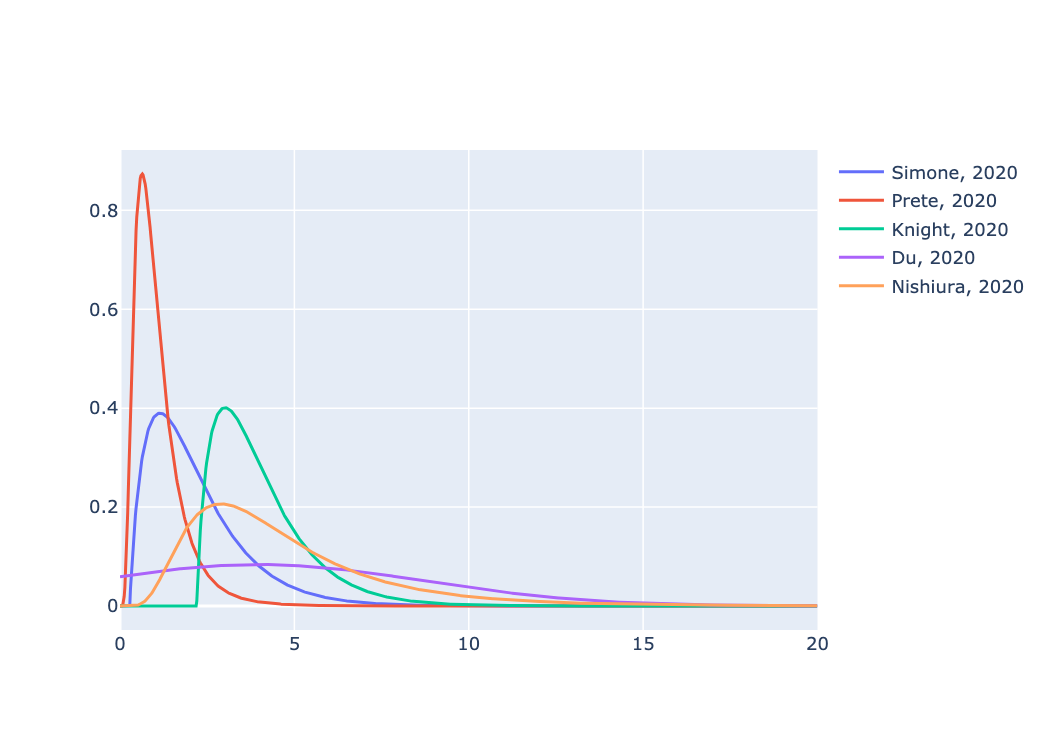
\includegraphics[width=\textwidth]{generated/images/serial-intervals-overview.png}
  \end{center}
  \caption{Referenced serial intervals}
  \label{fig:serial-intervals-overview}
\end{figure}

The previous serial intervals vary due to spatial and temporal differences in population composition and the strain of the virus.
From the local research made by \cite{majek2020}, it is estimated the SI of Covid-19 for Czech republic is 4-5 days, which is stated to be consistent with \cite{nishiura2020}. 
In the time of writing this thesis, more precise work on the SI of predominant delta mutation could not be found. 
Therefore we will stick with \cite{majek2020} and \cite{nishiura2020} and assume $\omega \sim LogNormal \left( \mu = 4.7, \sigma = 2.9 \right)$ as the source of truth.

\newpage
As we assumed $\omega$, we can easily compute $\bar{\Omega}$ and make an assumption about $a_{max}$.
Let's plot the $\bar{\Omega}$:

\begin{figure}[H]
  \begin{center}
    \includegraphics[width=\textwidth]{generated/images/data-1-Omega.png}
  \end{center}
  \caption{$\bar{\Omega}$}
  \label{fig:data-1-Omega}
\end{figure}

Given the previous figure, we can safely assume 
$a_{max} = 10$ as sufficient.

\section{Summary}

In this chapter, the situation was analyzed.
That means we investigated the available epidemic, population, and serial interval to use as a generation time $\omega$.
We also derived the formula for prevalence calculation, which depends on incidence $c$ and $\omega$.

For now, the only problem is the incidence $c$, for whom the observed values $Y_c$ are available.
There is a huge noisiness in the data, which can be overcome by using smoothing techniques.

The article \cite{elmousalami2020} compares deterministic methods as the moving average, weighted moving average, single exponential smoothing for forecasting Covid-19, while these methods may be used for smoothing too.
\cite{annunziato2020} draws attention to use smoothing methods carefully as some oscillations might remain in the input data from the improper data collection.

Therefore, it is crucial to devote sufficient time to choosing the proper smoothing technique.
The next chapter is dedicated to the inference of incidence estimation $\hat{c}$ from the observed incidence $Y_c$, i.e., denoise/smoothen $Y_c$ to $\hat{c}$. This part will be called \textit{the incidence model}.


\chapter{The incidence model}

In the most basic taxonomy of mathematical models, they can be split into two main categories: \textit{deterministic} and \textit{probabilistic}, also known as \textit{stochastic}. 
A big advantage of deterministic models is their straightforwardness and lower computational demands. 
On the other hand, they bring one huge pitfall - inferior options to display uncertainty, meaning it misses the idea of how certain we are about the value, especially in stochastic systems.
In the probabilistic modelling, the value is represented by its probability distribution, so the idea about certainty in the particular variable value is available.
The probabilistic modelling is based mostly on the Bayesian approach, named after Thomas Bayes\footnote{\url{https://en.wikipedia.org/wiki/Thomas_Bayes}}, the Reverend and philosopher, who brought foundation to the Bayes theorem we use today.


\section{Bayesian approach}

Contrary to the frequentist approach, the Bayesian way of thinking is more similar to how the human brain works. 
Usually, we humans have some prior belief about some unknown quantity or event. We update our belief whenever we obtain new evidence, forming the posterior.
The next time we obtain new evidence, this posterior is used as a new prior, and so forth, by this iterative manner.
Technically, every time someone asks us about our opinion about a quantity, we usually express our latest knowledge, i.e., the posterior.
Basically, the more evidence we have collected about the quantity over time, the stronger our belief about the value of that quantity is.

Let us imagine a toy example with coin tossing. 
Initially, before we toss the coin, we have no reason to think the coin is not fair, so we put our prior belief in tossing head to $50\%$ and tail to $50\%$ as well. 
Nevertheless, if we start tossing and obtaining 8 tails in a row, we may believe the coin is biased. 
In reality, we should toss the coin many (ideally infinitely many) times to confirm its fairness, but by doing this, we fall back to a frequentistic way of thinking. 
The Bayesian approach allows us to be "more subjective" regarding the evidence we obtained. 
Therefore, it better fits situations when only a few or uncertain data are available.

Formally, let $X$ be a random variable representing the unknown quantity of interest and $Y$ random variable for the observed quantity.
Therefore we can express $p(X)$ as a \textit{prior distribution} of the unknown quantity, and $p(Y)$ as a probability distribution of evidence.
\textit{Posterior distribution} can be expressed in terms of conditional probability such that $p(X | Y)$, meaning what the probability distribution of $X$ given we know/observe $Y$ is. 
This posterior can be obtained using the \textit{Bayes theorem}:

\begin{equation}\label{eq:bayes-theorem}
p( X | Y ) = \frac{p( Y | X ) p(X)}{p(Y)} \text{,}
\end{equation}

\noindent
where the $p( Y | X )$ is called the \textit{likelihood}.
Note that the likelihood is dual to posterior, i.e., it is a probability distribution of evidence given the $X$.
In practice, the probability distribution of evidence $p(Y)$ is usually not directly available, but can be obtained by marginalization over the $X$, referred as a \textit{normalizing constant} $\eta$ or \textit{marginal likelihood}:

\begin{equation}\label{eq:bayes-normalizing-const}
  p(Y) = \eta = \int_\mathcal{X} p( Y | X ) p(X) dX \text{,}
\end{equation}

\noindent where $\mathcal{X}$ is a domain of $X$.

Unfortunately, the integral in equation \eqref{eq:bayes-normalizing-const} is not usually easily analytically tractable.
This makes the Bayesian approach quite more complex than frequentist.
However, during the last decades, there was a huge leap in the development of inference methods capable of overcoming this problem (more in Section \ref{sec:monte-carlo}). 
Choosing the proper method depends on the defined model \cite{pfeffer2016}, so it will be convenient to begin with the probabilistic incidence model first.


In terms of the Bayes theorem \eqref{eq:bayes-theorem}, $Y$ will be represented just by the observed incidence $Y_c$, and $X$ will represent the set of internal parameters to infer.
Moreover, we assume also a set of hyperparameters $Z$ such that the Bayes theorem can be rewritten as:

\begin{equation}\label{eq:bayes-theorem-customized}
  p( X | Y_c, Z ) = \eta^{-1} p( Y_c | X ) p(X | Z) \text{,}
\end{equation}

\noindent
where $\eta$ is the \textit{normalizing constant} as defined in \eqref{eq:bayes-normalizing-const}, $p(X | Z)$ is the prior, and $p( Y_c | X )$ is likelihood.
To define the prior, we have to know the parameter set $X$, which depends on the likelihood probability, so let us define the likelihood first.


\section{The likelihood}

As the daily incidence is a discrete count variable, the discrete probabilistic distributions are considered a likelihood. One of the first suggestions might be the \textit{Poisson distribution}.
Unfortunatelly, random variable $X$ following the Poisson distribution with parameter $\lambda$ has very strong assumption about expected value and variance $\lambda = \mathbb{E}\left[ X \right] = \text{Var} \left[ X \right]$, which is not our case as the Figure \ref{fig:largest-cities-incidence} shown high overdispersion.
Therefore we need better parametrization options.
This can be achieved by taking Poisson distribution and using Gamma distribution as a conjugate prior:

\begin{equation}\label{eq:poisson-gamma-conjugate}
  \begin{split}
    y_c & \sim \text{Poisson}(\lambda) \\
    \lambda & \sim \text{Gamma}(r, \frac{p}{1 - p})
  \end{split}
\end{equation}

It can be proved \cite{barry2020} that this corresponds to the \textit{negative binomial distribution}:

\begin{equation}\label{eq:neg-bin-distribution}
  y_c \sim \text{NegBin}\left( r, p \right),
\end{equation}

\noindent
where $r$ is the number of successful Bernoulli trials and $p$ is the probability of success in one trial. The negative binomial distribution as a likelihood for incidence was also used by \cite{simone2020}, \cite{wallinga2004}, \cite{alzahrani2018} and \cite{manevski2020}.

In our case, we need to parametrize over the mean $\mu$ of the resulting random variable.
Therefore we will reparametrize $\mu = \frac{r(1 - p)}{p}$, and as $r$ directly corresponds to the first parameter of Gamma distribution in \eqref{eq:poisson-gamma-conjugate}, which is usually called \textit{shape} and denoted $\alpha$, we will use $\alpha = r$:

\begin{equation}\label{eq:neg-bin-distribution-reparametrized}
  y_c \sim \text{NegBin}\left( \mu, \alpha \right)
\end{equation}

% Then, the probability mass function of such negative binomial distribution as the likelihood for incidence is:

% \begin{equation}
% f \left( y_c; \mu, \alpha \right) = \frac{\Gamma \left( \alpha + y_c \right) }{y_c! \Gamma \left( \alpha \right)} \left( \frac{\alpha}{\mu + \alpha} \right)^{\alpha} \left( \frac{\mu}{\mu + \alpha} \right)^{y_c} \text{,}
% \end{equation}

% \noindent
% where $\mu \geq 0$ is the mean and $\Gamma$ is the \textit{gamma function} and $\alpha$ is the first parameter of the conjugate prior Gamma.

We assume the distribution of incidence will have a distinctly more heavy tail for the values less than $\mu$, which is the case of $\alpha$ values closer to zero.
Therefore $\alpha$ is assumed to be distributed exponentially:

\begin{equation}\label{eq:alpha-prior}
	\alpha \sim \text{Exponential} \left( \lambda_{\alpha} \right)
\end{equation}

\noindent
where $\lambda_{\alpha}$ is a rate parameter of that exponential distribution, considered hyperparameter in our model.

As the previous analysis shown significant correlation between mean and variance, and the seasonal decomposition in Subsection \ref{sec:seasonality-decomposition} shown rather the multiplicative effect between trend, seasonal component and residual, the logarithmic transformation $\log \left( \mu \right) = \theta$ is considered \cite{cialdella2020}.
The following plot shows the original data before and after the logarithmic transformation\footnote{Created by Snippet \ref{snip:incidence-log-transform-plot}}:

\begin{figure}[H]
  \begin{center}
    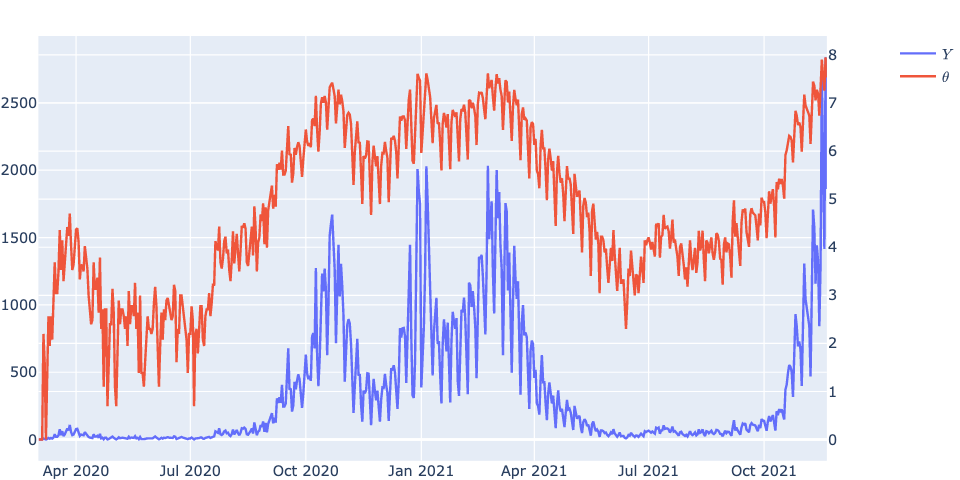
\includegraphics[width=\textwidth]{generated/images/incidence-log-transform.png}
  \end{center}
  \caption{Log transformation of daily incidence}
  \label{fig:incidence-log-transform}
\end{figure}

Moreover, the transformed trends are now linear, which implies the exponential growth in the original data.
The likelihood can be finally defined as:

\begin{equation}\label{eq:likelihood-first}
  p( y_c | \theta, \alpha )
\end{equation}

The prior for $\alpha$ was already stated by \eqref{eq:alpha-prior}.
The $\theta$ requires further introspection to choose a proper distribution.


\section{The analysis of \texorpdfstring{$\theta$}{Lg}}
\label{sec:theta-analysis}

After the transformation, $\theta \in \mathbb{R}$.
This means the multiplicative effect of mean and variance was changed to additive (See Figure \ref{fig:incidence-log-transform}) resulting in more homoscedastic random variable, which is convenient because the more homoscedastic the random variable is, the more constant variance it has, i.e., approaches weak stationarity.
The above can be verified by first-order detrending/decumulation\footnote{See Snippet \ref{snip:theta-diff-plot}} of $\theta$, to obtain differences $\Delta \theta$, with succesive application of $\Delta \theta_t = \theta_{t+1} - \theta_{t}$:

\begin{figure}[H]
  \begin{center}
    \includegraphics[width=11cm]{generated/images/theta-diff.png}
  \end{center}
  \caption{The plot of $\Delta \theta$}
  \label{fig:theta-diff}
\end{figure}

Naturally, we could check the normality of the whole data, as we did in the case of stationarity, but practically, we will use just specific time windows of size $T_w$, in which the normality of the data will be assumed, therefore it will be more meaningful to verify normality for those windows.
In our case, we randomly picked three samples of time window $T_w = 50$ as the following figure presents\footnote{Created by Snippet \ref{snip:theta-diff-sample-windows-plot}}:

\begin{figure}[H]
  \begin{center}
    \includegraphics[width=11cm]{generated/images/theta-diff-sample-windows.png}
  \end{center}
  \caption{The referenced windows for taking samples of $\Delta \theta$}
  \label{fig:theta-sample-windows}
\end{figure}

This means that for the inference of incidence up to time $t$, we will assume data only from the interval $[t - T_w, t]$, i.e., assuming each sample from time period less than $t - T_w$ is irrelevant.
This will also help to reduce computational complexity.

Let's explore the distribution of those samples for confirmation of normality. 
For visual testing of normality, histogram, Q-Q and ECDF/CDF plots may be considered.
Let's start with histograms\footnote{Created by Snippet \ref{snip:theta-diff-histogram}}:

\begin{figure}[H]
  \begin{center}
    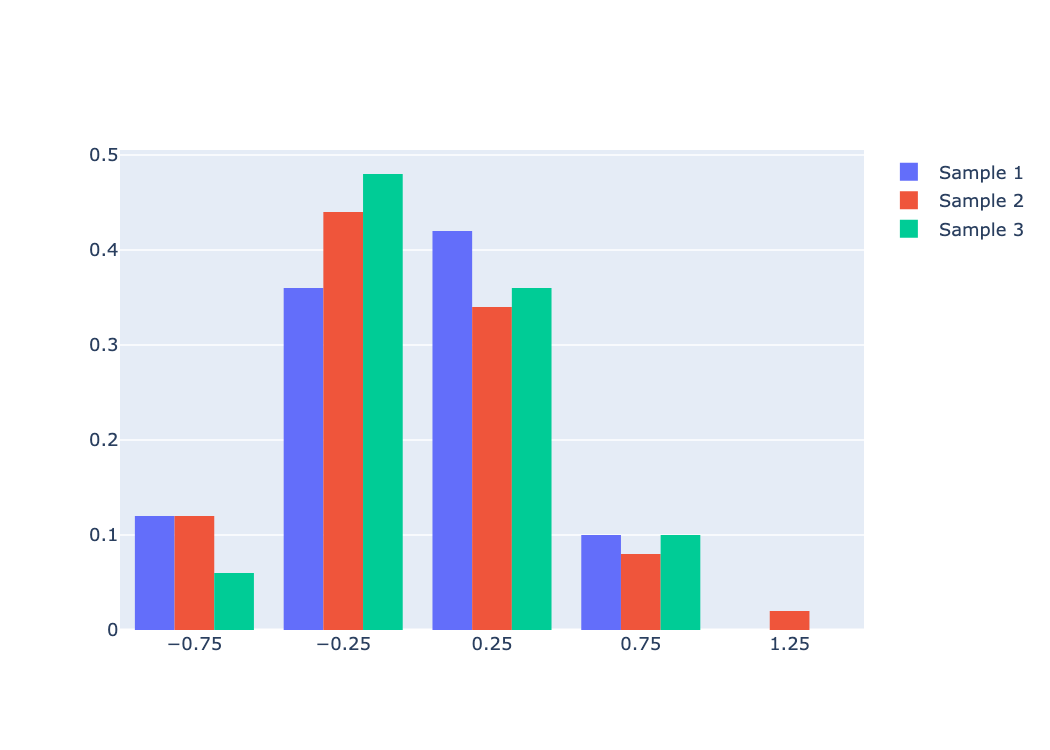
\includegraphics[width=11cm]{generated/images/theta-diff-histogram.png}
  \end{center}
  \caption{The histogram of chosen $\Delta \theta$ samples}
  \label{fig:theta-diff-histogram}
\end{figure}

From the histogram, the normality is not very obvious.
The main pitfall of a histogram is the problem of choosing the proper bin size, which we may think of as some hyperparameter.
Too narrow bin size means a lot of bins, which require a lot of data.
Too wide bins, on the other hand, too wide bins end with few bins in the visualization, and we might oversee gaps in the data as in our case.
The Q-Q plot is better in this way because it can be assumed as a non-parametric visualization, where we see how all data points fit the normal distribution\footnote{Created by Snippet \ref{snip:theta-diff-qq-plot}}:

\begin{figure}[H]
  \begin{center}
    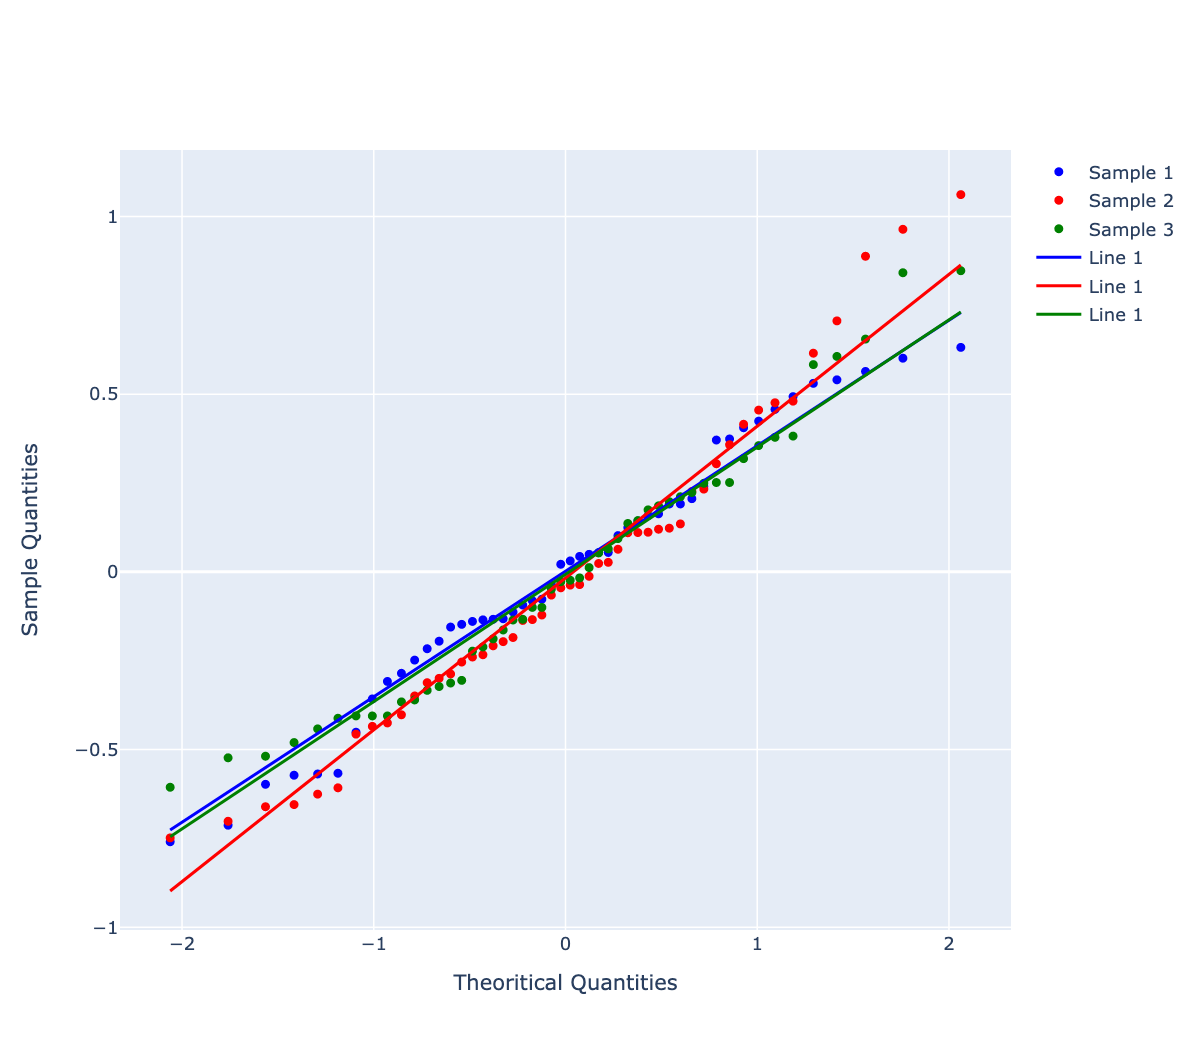
\includegraphics[width=11cm]{generated/images/theta-diff-qq.png}
  \end{center}
  \caption{Quantile-Quantile plot of $\Delta \theta$ samples}
  \label{fig:theta-diff-qq}
\end{figure}


This may finally remind the normally distributed data because the closer the points are to the line, the more normal distribution is approached by the data.

The next plot\footnote{Created by snippet \ref{snip:theta-diff-ecdf-plot}} visualizes the \textit{empirical cumulative distribution function} (ECDF) based on $\Delta \theta$ and CDF for the theoretical normal distribution based on the summary statistics of $\Delta \theta$:

\begin{figure}[H]
  \begin{center}
    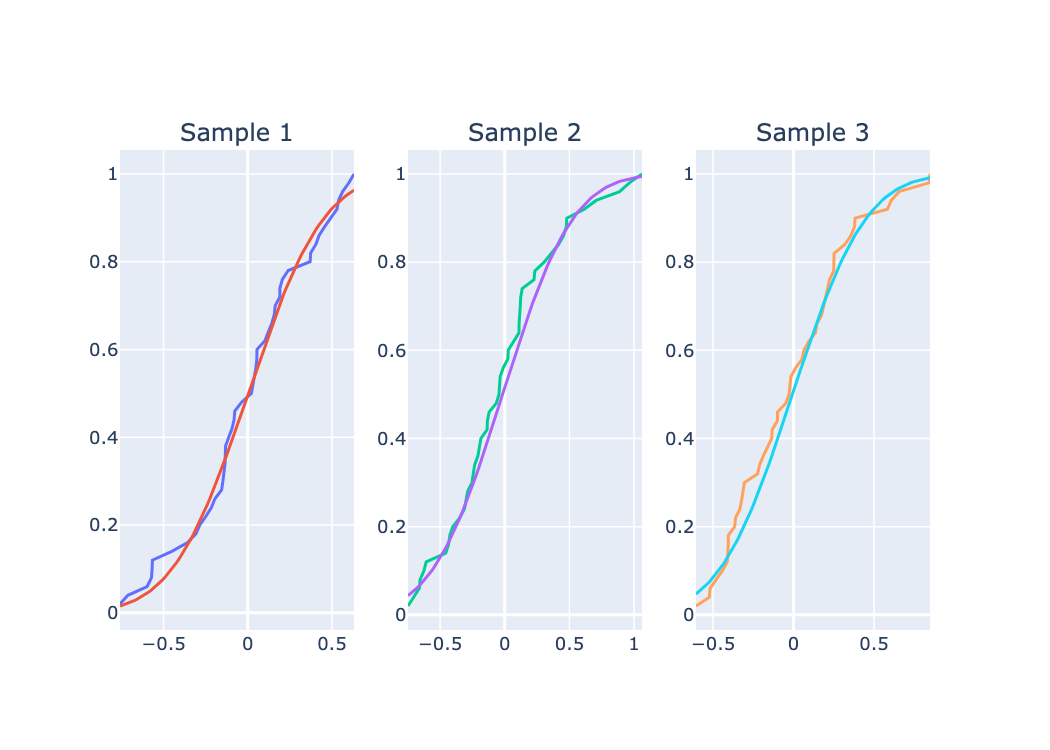
\includegraphics[width=11cm]{generated/images/theta-diff-ecdf.png}
  \end{center}
  \caption{Empirical and theoretical CDFs of $\Delta \theta$ samples}
  \label{fig:theta-diff-ecdf}
\end{figure}

The previous visuals might evoke normally distributed data for some individuals, but visual checks might be misleading; therefore, they should not be sufficient for statistical modelling.
Visual checks can be complemented with statistical tests.
The statistics provides several non-parametric normality tests.
In our case, Kolmogorov-Smirnov, Lilliefors, and Shapiro-Wilk tests were performed.

\input{generated/tables/theta-diff-ks-test}
\input{generated/tables/theta-diff-lilliefors-test}
\input{generated/tables/theta-diff-shapiro-wilk-test}

The strongest result is noted in the Lilliefors test, then the Shapiro-Wilk test, and the worst result is from the Kolmogorov-Smirnov test.
The research of \cite{razali2011} concludes the Shapiro-Wilk test to be the most powerful normality test and the Kolmogorov-Smirnov test to the least powerful (Kolmogorov-Smirnov, Shapiro-Wilk, Anderson-Darling, and Lilliefors tests were compared).
According to this research and the fact we use limiting window $T_w$, the assumption about normally distributed $\theta$ can be made.
Moreover, as the $\theta$ is actually a function of time $\theta(t)$, we can model its prior as a \textit{Gaussian process}.
Let us introduce a very brief theory for Gaussian processes in the following section, and then we will continue with the prior for $\theta$ in the following section.


\section{Gaussian process}

Gaussian process (GP) is a stochastic process that is used to directly infer from data over a finite set of functions.
Basically, it is a probability distribution over set of functions which follow \textit{joint (multivariate) Gaussian distribution} \cite{frigola2015}:

\begin{equation}
    \begin{bmatrix}
      f(x) \\ f(x_\star)
    \end{bmatrix} \sim \text{MN}\left(
    \begin{bmatrix}
      m(x) \\ m(x_\star)
    \end{bmatrix},
    \begin{bmatrix}
      k(x, x) & k(x, x_\star) \\ 
      k(x, x_\star)^\top & k(x_\star, x_\star) \\ 
    \end{bmatrix}
  \right)
\end{equation}

where $f(x)$ is basically internal state inferred from the input data (trained model in terms of machine learning), and $f(x_\star)$ is a function we want to predict in $x_\star$.

For simplicity, we denote previous as:

\begin{equation}
  f(x) \sim \text{GP} \left( m \left( x \right), k \left( x, x' \right) \right)
\end{equation}

where $m \left( x \right)$ and $k\left( x, x' \right)$ are 
the specifying\footnote{GP is specified only with these two functions} mean and
covariance functions respectively.
For those functions the following apply \cite{rasmussen2004}:

\begin{equation}
\begin{split}
  & m(x) = \mathbb{E} \left[ f(x) \right] \\
  & k \left( x, x' \right) = \mathbb{E} \left[ 
    \left( f \left( x \right) - m \left( x \right) \right)
    \left( f \left( x' \right) - m \left( x' \right) \right)
  \right]
\end{split}
\end{equation}

The covariance function is often called \textit{kernel function} which is actually \textit{Mercer kernel}, also called \textit{positive-definite kernel} \cite{murphy2021}, measuring how two inputs $x$ and $x'$ are similar.
This requires the kernel to be symmetric, i.e., $k \left( x, x' \right) = k \left( x', x \right)$.
These kind of function are also called \textit{smoothing functions/kernels} \cite{martin2016}.


\section{The prior of \texorpdfstring{$\theta$}{Lg}}

The prior of $\theta$ is assumed to be a Gaussian process:

\begin{equation}
  \theta(t) \sim \text{GP}(m, k(t, t^\prime))
\end{equation}

According to the Figure \ref{fig:incidence-log-transform}\footnote{Created by Snippet \ref{snip:incidence-log-transform-plot}}, the linear trend between points should be sufficient, therefore let $m$ be defined as:

\begin{equation}
m(t) = b + a t
\end{equation}

where the prior distributions for $a$ and $b$ are assumed $a \sim N \left( \mu_a, \sigma_a \right)$ and $b \sim N \left( \mu_b, \sigma_b \right)$.
Someone may argue why there is no restriction such as $a \geq 0$ and for $b$ such that $m(t) \geq 0$, but if $\theta < 0$, then $0 \leq e^{\theta} < 1$, which are still valid values for the $\mu$ parameter of our likelihood.
Basically, we let the $\theta(t)$ move free in its whole space $\mathbb{R}$ because the exponential transformation always keeps $\mu \geq 0$.

For the sake of simplicity, as a kernel we chose one of the well-known and most basic kernels, \textit{Gaussian kernel}, also called \textit{squared exponential kernel} or \textit{radial basis function (RBF) kernel} defined as (for univariate observations, which is our case):

\begin{equation}
k_{RBF} \left( t, t'; \ell \right) = \exp \left[ -\frac{(t - t')^2}{2\ell^2} \right]
\end{equation}

where $\ell$ is the \textit{length scale} hyperparameter, known also as \textit{bandwidth} (denoted $\sigma$ in some literature). 
This hyperparameter is distance which we expect differences to matter, in our case\footnote{See snippet \ref{snip:hyperparameters}} $\ell = 7$ as we observed weekly seasonality.


\section{Monte Carlo simulation}
\label{sec:monte-carlo}

The simulation itself is a relatively old technique for solving analytically intractable problems. 
The first such problem considered is the \textit{Buffon's needle problem}\footnote{\url{https://en.wikipedia.org/wiki/Buffon\%27s_needle_problem}} from 1733. 
The problem is defined as the probability of the needle of length $l$ dropped onto the floor, represented by parallel strips of distance $d$, crossing the line between two adjacent strips.
The analytical solution was discovered in 1777; however, the simulation can be done by dropping the needles on the floor and counting the intersections to calculate the probability in a frequentist way.

Massive development in simulation techniques naturally came with the development of computers, especially during the Los Alamos research \cite{metropolis1987}, where \textit{Monte Carlo simulation}\footnote{In fact, the name Monte Carlo refers to the city in Monaco, which is famous for its casinos. In the casinos, generally, the probability and randomness together play a significant role, just like in the Monte Carlo simulation.} was invented to solve the nuclear fission problem.

The whole idea started when Stan Ulam\footnote{\url{https://cs.wikipedia.org/wiki/Stanis\%C5\%82aw_Ulam}} was trying to compute odds in solitaire.
He tried to solve the problem analytically, but he later realized the problem could be solved in a much simpler way, just by uniformly sampling layouts of cards in hand and counting the number of successful games.
This is how the \textit{random sampling} was born.

John von Neumann\footnote{\url{https://cs.wikipedia.org/wiki/John_von_Neumann}} was interested in Ulam's idea. He saw a big potential for solving intractable problems in physics.
Unfortunately, in physics, there are many problems where we know some distributions in theory, but they are difficult to sample from, so von Neumann later invented \textit{rejection sampling} \cite{beichl2000}, which was a foundation for the future development of Monte Carlo techniques.

Monte Carlo methods can be used for various purposes, mostly used for integration and optimizations problems, for example, in the Bayesian inference is used for \cite{andrieu2003}:

\begin{itemize}
  \item \textit{Normalization} - computing posterior $p(X | Y)$ from:
    \begin{equation}
      p(X | Y) = \frac{p(Y | X) p(X)}{\int_{\mathcal{X}} p(Y | X^\prime) p(X^\prime) dX^\prime}
    \end{equation} \\
    where the denominator is the normalizing constant $\eta$ which is usually intractable.
  \item \textit{Marginalization} - computing marginal probability $p(Y)$ from the joint distribution $p(X, Y)$:
    \begin{equation}
      p(Y) = \int_{\mathcal{X}} p(X, Y) dx
    \end{equation} \\
    This is basically just a subtask of the normalization mentioned before.
  \item \textit{Expectation} - to calculate expected value as in \eqref{eq:random-sampling-expectation}
\end{itemize}

In the following sections, the evolution of the algorithmic approach is described.
It is not necessary for further understanding, but it covers the theoretical background of MCMC, which is utilized in this thesis.
If the reader is interested only in the particular solution, he may skip directly to the Section \ref{sec:pymc3}.


\subsection{Random sampling}

Let imagine we have a random variable $x \in \mathcal{X}$ distributed according to $p$ and we are interested in its expected value $\mathbb{E}_p$.
The usual approach would be:

\begin{equation}\label{eq:random-sampling-expectation}
  \mathbb{E}_{p}\left[ f(x) \right] = \int_{\mathcal{X}} p \left( x \right) f \left( x \right) dx
\end{equation}

But in many cases, the $p$ is not directly observable, as we usually do not have all the possible data.
The Monte Carlo may approach this value by generating $n$ independent identically distributed random samples $x_i$ (if sampling from $f$ is possible) from domain $\mathcal{X}$ to form a sample mean of that unknown quantity:

\begin{equation}
  \hat{\mu}_n = \frac{1}{n} \sum_{i=1}^{n} f_{x_i}
\end{equation}

According to the unknown quantity above, this is its \textit{unbiased Monte Carlo estimator}, i.e., the estimator of the expected value. 
As $n \to \infty$, from the law of large numbers, we can state $\hat{\mu}_{\infty} = \mathbb{E}_{\pi}\left[ f(x) \right]$, therefore for very large $n$ it holds $\hat{\mu}_n \approx \mathbb{E}_{\pi}\left[ f(x) \right]$.

In this approach, the samples are genuinely random, meaning independent of each other, hence the name \textit{random sampling}.
The main pitfall of random sampling is its computational inefficiency, i.e., we need $n$ to be a very large number to be sure the samples sufficiently cover $\mathcal{X}$, even for highly improbable values of $x_i$, i.e., $\pi(x_i) \approx 0$.


\subsection{Rejection sampling}
\label{sec:rejection-sampling}

In rejection sampling, the basic assumption is we have \textit{target probability distribution} $f$ for which we want to estimate some quantity.
Unfortunately, we cannot sample from $f$, or the sampling is somehow complicated.
Rejection sampling can overcome this by sampling from other distribution related to the $f$ and easy to sample from, the \textit{proposal distribution} $g$.
The algorithm proceeds as follows \cite{beichl2000}:

\begin{enumerate}
  \item Sample proposal $x \sim g(x)$
  \item Generate $u \sim \text{Uniform}(0, 1)$
  \item If $u < \frac{f(x)}{M g(x)}$ accept $x$
  \item Go to step 1
\end{enumerate}

The sample $x$ from a proposal distribution $g$ is generated in the first step.
Then $u$ is randomly chosen such that $u \in [0, 1)$.
As the condition in \eqref{eq:rejection-sampling-cond} must be kept, then $\frac{f(x)}{M g(x)} \leq 1$.
The ratio $\frac{f(x)}{M g(x)}$ closer to $1$ means the $x$ was generated from higher density region.
Consequently, when this ratio is closer to $0$, it means the value sampled is unlikely.
The higher the ratio is, the more likely we accept $x$, and after a sufficient amount of steps (or accepted samples), the algorithm might be terminated.
The acceptance in this algorithm is related to the term \textit{acceptance rate}, which is the ratio of the number of accepted samples and the number of total samples generated.

The algorithm depends on a very limiting condition:

\begin{equation}\label{eq:rejection-sampling-cond}
  M \geq \frac{f(x)}{g(x)}, \forall x
\end{equation}

This means we have to choose sufficiently large $M$ such that we are ensured the $M g(x)$ for every $x$ creates an envelope around the whole $f$.
However, if we pick $M$ too high, we will reject most samples, i.e., we will achieve a very low acceptance rate, and the simulation will be computationally inefficient.

The condition \eqref{eq:rejection-sampling-cond}, and therefore the problem with acceptance rate, may be overcomed with the employment of some type of memory.


\section{Markov Chain Monte Carlo}

\textit{Markov Chain Monte Carlo} (MCMC) is a class of algorithms solving a problem with sampling from a \textit{target probability distribution} $f$ in a more efficient way than random and rejection sampling mentioned before.
The basic principle is to walk through distribution similarly to random sampling, but we also utilize the previously generated samples.
These samples are forming a sequence with a Markov property, hence the name \textit{Markov chain}.

To recall, Markov property states the future state $X_{t+1}$ is only dependent on the current state $X_t$, formally in the discrete-time:

\begin{equation}
  p(X_{t+1} | X_t, X_{t - 1}, \dots, X_0) = p(X_{t+1} | X_t)
\end{equation}

The Markov chain is a sequence of values, where this rule applies for each value in that chain (except the first one).
MCMC utilizes Markov chain as a store of produced samples, where each new sample generated is dependent on the previous.


\subsection{Metropolis algorithm}

The algorithm is named after his inventor, Nicholas Metropolis\footnote{\url{https://en.wikipedia.org/wiki/Nicholas_Metropolis}}, and is the very first Monte Carlo algorithm utilizing Markov chains \cite{metropolis1953}.
Let imagine we are interested in the theoretical probability distribution $f(x)$ of some parameter $x$, which is not easily tractable (same as in the case of rejection sampling).
The idea is to gradually generate the $x^\prime$ parameter into the sequence forming Markov chain.
The generation is done with a proposal distribution $g(x^\prime | x_{i})$ conditionally dependent on the last sample $x_{i}$ in the forming Markov chain\footnote{To be more specific, since the $g$ is conditionally dependent only on the last sample, it is so-called first-order Markov chain} $X_{0:i}$.
Assume input $x_0$ and $i = 0$, then the algorithm process itself might be summarized in the following steps:

\begin{enumerate}
  \item Generate proposal $x^\prime \sim g(x^\prime | x_{i})$
  \item Compute $\alpha$ according to \eqref{eq:metropolis-alpha}
  \item Generate $u \sim \text{Uniform}(0, 1)$
  \item Set $x_{i+1} \leftarrow \begin{cases}
    x^\prime, & \text{ if } u \leq \alpha,\\
    x_{i}, & \text{ otherwise}
    \end{cases}
    $
  \item Set $i \leftarrow i + 1$ and go to \textit{step 1}
\end{enumerate}

In the first step, the parameter proposal $x^\prime$ is generated from proposal distribution $g$.
The second step assumes computation of the \textit{acceptance probability} $\alpha$:

\begin{equation}\label{eq:metropolis-alpha}
  \alpha = \min \left(1, \frac{f(x^\prime)}{f(x_{i})}\right)
\end{equation}

The ratio $\frac{f(x^\prime)}{f(x_{i})}$ expresses how many times $x^\prime$ is more probable than $x_{i}$.
This probability is then compared with uniformly generated $u \in [0, 1)$. 
Note the similarity with rejection sampling defined in Subsection \ref{sec:rejection-sampling}.
This may look a little bit counterintuitive because of the possibility of accepting $x^\prime$ with a lower probability than $x_{i-1}$. However, the whole idea of acceptance probability is to explore further areas of state space to prevent getting stuck in a local minimum.
Basically, the probability of transition into a particular state is proportional to the probability of that state, i.e., the states with higher probabilities are preferred.

For the initial state $x_0$, we usually put our initial prior, which affects the convergence speed - the more accurate the prior is, the faster the convergence is.
After a sufficient amount of steps, the Markov chain should reach the stationary target distribution $f(x)$.

One of the primary pitfalls of the Metropolis algorithm is its inability to use asymmetric proposal distributions.
Hasting's modification solves this issue.


\subsection{Metropolis-Hastings algorithm}

Metropolis-Hastings algorithm is a generalization of the Metropolis algorithm allowing to sample from asymmetric proposal distributions.
This modification was first introduced by Wilfred K. Hastings in 1970, only by using the following acceptance probability $\alpha$:

\begin{equation}\label{eq:metropolis-hastings-alpha}
  \alpha = \min \left(1, \frac{f(x^{\prime})}{f(x_{i})} \frac{g(x_{i} | x^{\prime})}{g(x^{\prime} | x_{i})}\right)  
\end{equation}

The difference lies only in adding multiplication by the ratio $\frac{g(x_{i} | x^{\prime})}{g(x^{\prime} | x_{i})}$ which is originally derived from the detailed balance principle \cite[Chapter 11]{owen2013}:

\begin{equation}
  p(x^\prime | x) p(x) = p(x | x^\prime) p(x^\prime)
\end{equation}

Although the Metropolis algorithm was generalized to use asymmetric proposals, it is still relatively inefficient in exploring state space, in the same way as the Metropolis algorithm, especially for multidimensional problems, because of its randomness in proposal distribution.


\subsection{Boltzmann factor}
\label{sec:boltzmann-factor}

In many cases, the ratio of two probabilities (as was seen in \eqref{eq:metropolis-alpha} and \eqref{eq:metropolis-hastings-alpha}) is not computationally very feasible because of the possibility of division with tiny numbers (possible zero division).
Therefore, for practical purposes, the physical analogy with \textit{Boltzmann distribution} is being used \cite{murphy2021}.
The Boltzmann distribution represents a probability of particular state $x$ of a physical system as this proportionality:

\begin{equation}\label{eq:boltzmann-factor-prop}
  p(x) \propto \exp \left( -\frac{E(x)}{kT} \right),
\end{equation}

where $E(x)$ is energy of $x$, $T$ is temperature and $k$ is Boltzmann's constant\footnote{\url{https://en.wikipedia.org/wiki/Boltzmann_constant}}, $\exp \left( -\frac{E(x)}{kT} \right)$ is called the \textit{Boltzmann factor}.

Since $k$ is always constant and we do not need to simulate exact physical result of particles, we getting rid of $k$ and proportionality.
$T$ is usually used in the \textit{simulated annealing} where we decrease $T$ gradually with time (more on this in \cite[Chapter 8]{murphy2021}), however, in this case we do not employ that, i.e., assuming $T = 1$, then:

\begin{equation}\label{eq:boltzmann-factor-prob}
  p(x) = \exp \left( -E(x) \right)
\end{equation}

And analogically:

\begin{equation}\label{eq:boltzmann-factor-neg-log}
  E(x) = -\log p(x)
\end{equation}

This basically states lower the energy $E(x)$ of $x$ is, the higher the probability of $x$.
In statistics, $E$ is in this case called \textit{negative log probability}.
Now we can derive the formula for the ratio of probabilities:

\begin{equation}
  \frac{p(x)}{p(y)} = \exp \left( -(E(x) - E(y)) \right) = \exp \left( E(y) - E(x) \right)
\end{equation}

For example, the acceptance probability \eqref{eq:metropolis-alpha} for Metropolis can be rewritten:

\begin{equation}
  \begin{split}
    \alpha &= \min \left(
    1, 
    \exp\left( 
      E(x_{i}) - E(x^\prime)
    \right) 
  \right) \\
  & = \min \left(
    1, 
    \exp\left( 
      \log f(x^\prime) - \log f(x_{i})
    \right) 
  \right)
  \end{split}
\end{equation}

Similarly for the ratio in acceptance probability \eqref{eq:metropolis-hastings-alpha} of Metropolis–Hastings:

\begin{equation}
  \exp \left( \log f(x_{i}) + \log g(x^{\prime} | x_{i}) - \log f(x^\prime) - \log g(x_{i} | x^{\prime}) \right)
\end{equation}

% \begin{equation}\label{eq:metropolis-hastings-alpha}
%   \alpha = min\left(1, \frac{f(x^{\prime})}{f(x_{i})} \frac{g(x_{i} | x^{\prime})}{g(x^{\prime} | x_{i})}\right)  
% \end{equation}

\subsection{Hamiltonian Monte Carlo}

\textit{Hamiltonian Monte Carlo} (HMC) is another Metropolis-based algorithm, but it utilizes physical analogy to generate proposals more efficiently as the gradient of proposal distribution is available \cite{betancourt2018}.

It started with the Hybrid Monte Carlo paper \cite{duane1987}, which utilized Monte Carlo to understand the structure of atoms. 
Radford Neal lately recognized the potential of this method during his focus on Bayesian neural networks within his doctoral thesis \cite{neal1995}. 
\cite{mackay2003} started to use term \textit{Hamiltonian Monte Carlo} under which this method is known to this day.
Neal, again, did an extensive review of HMC \cite{neal2011}.
However, HMC had to wait until the advent of highly efficient computational software was available, allowing its practical usage.

In Hamiltonian dynamics, state is characterized by the \textit{position vector} $x$ and the \textit{momentum vector} $p$, both are $d$-dimensional, hence $2d$-dimensional state.
We usually measure total energy in the system by the function of the state $H(x, p)$ called \textit{Hamiltonian}.
The Hamilton’s equations describe how position $x$ and $p$ change according to time $t$ by the partial derivatives \cite{neal2011}:

\begin{equation}
  \frac{\partial x_i}{\partial t} = \frac{\partial H}{\partial p_i}
\end{equation}

\begin{equation}
  \frac{\partial p_i}{\partial t} = - \frac{\partial H}{\partial x_i}
\end{equation}

where $i = 1, \dots, d$ is the dimension.
The Hamiltonian $H$ can be thought of as total energy in the whole system, i.e., the sum of \textit{potential energy} $U$ and \textit{kinetic energy} $K$:

\begin{equation}
  H(x, p) = U(x) + K(p)
\end{equation}

The $U$ corresponds to the equation \eqref{eq:boltzmann-factor-neg-log}, i.e., is assumed as negative log probability density of posterior $f(x)$ we want to sample from:

\begin{equation}
  U(x) = -\log f(x)
\end{equation}

The lower the probability $f(x)$ is, the higher energy $U(x)$ we obtain. 
Then we can rewritte partial derivative for momentum $p$ as:

\begin{equation}
  \frac{\partial p_i}{\partial t} = - \frac{\partial U}{\partial x_i}
\end{equation}

Kinetic energy $K(p)$ in multidimensional fashion is, according to physics, calculated as:

\begin{equation}
  K(p) = \frac{p^{\top} M^{-1} p}{2}
\end{equation}

where $M$ is symmetric, positive-definite mass matrix (often scalar-scaled identity matrix \cite{neal2011}).
With previous knowledge, the Hamiltonian equation for position (parameters) $x$ can be rewritten as:

\begin{equation}
  \frac{\partial x_i}{\partial t} = \frac{p_i}{m_i}
\end{equation}

The discretization is a necessary step in terms of solving Hamiltonian equations by computers.
There are several methods of discretization, where the best-known is probably \textit{Euler's method}\footnote{\url{https://en.wikipedia.org/wiki/Euler_method}}.
Unfortunately, in the case of Hamiltonian equations, the Euler method is not performing too accurately \cite[Chapter 5]{neal2011}.
As the one partial equation is dependent on another, HMC approaches derivatives with the \textit{leapfrog method} (or \textit{leapfrog intergration}) which is simple for implementation \cite{betancourt2018}, but very efficient.
The discretized equations approach the integration by interleaving 1/2 step $\epsilon$ to update the internal HMC state (vectors $x$ and $p$) as follows:

\begin{equation}
  p_i \left(t + \frac{\epsilon}{2} \right) = p_i(t) - \frac{\epsilon}{2} \frac{\partial U}{\partial x_i} (x(t))
\end{equation}

\begin{equation}
  x_i(t + \epsilon) = x_i(t) + \epsilon \frac{p_i \left(t + \frac{\epsilon}{2} \right)}{m_i}
\end{equation}

\begin{equation}
  p_i(t + \epsilon) = p_i \left( t + \frac{\epsilon}{2} \right) - \frac{\epsilon}{2} \frac{\partial U}{\partial x_i} \left( x \left( t + \epsilon \right) \right)
\end{equation}

These equations are applied $L$ times, where $L$ is the number of leapfrog steps. 
As $\epsilon$ is the size of a step, then $x(t + L \epsilon)$ is the final position we obtain after leapfrog integration.
At the end of the step, the HMC approaches similarly as Metropolis algorithm, except the acceptance probability $\alpha$ is computed from the Hamiltonian $H$, employing Boltzmann factor (\eqref{eq:boltzmann-factor-prop}):

\begin{equation}
  \alpha = \min \left( 1, \exp \left( H(x(t), p(t)) - H(x(t + L \epsilon), p(t + L \epsilon)) \right) \right)
\end{equation}

Although the algorithm is much more complex than the Metropolis-Hastings algorithm, i.e., the one iteration of HMC takes longer than MH, HMC usually reaches stationary distribution after fewer iterations as the proposal moves according to the gradient, and not randomly as in the case of MH.


\subsection{No U-Turn Sampler}
\label{sec:nuts}

The \textit{No U-Turn Sampler} (NUTS) was first introduced in 
paper \cite{hoffman2011} as an heuristic for HMC. 
In HMC, parameters $L$ and $\epsilon$ have to be tuned. 
This might cause several problems when finding proper values for demanding convergence.
According to \cite{betancourt2018}, if the integration trajectory is too short (i.e., low $L\epsilon$), we are not taking full advantage of gradient and rather approach random sampling, on the other hand, if it is too long (i.e., too high $L\epsilon$), the algorithm is computationally inefficient, because it may lead to often returns, in this case called U-turns.

NUTS solves this problem by expanding both sides of the trajectory, i.e., not only taking steps forward, as HMC does, but also backward.
This allows comparing $x$ and $p$ on both expanding sides to decide when to terminate the leapfrog integration.
This termination usually happens when both sides of expanding trajectory begin to approach each other.
This means we have reached the maximum possible width of energy level; thus, the further expansion is resource wasting.
For additional information and nice visualizations of MH, HMC, and NUTS, please see \cite{mcelreath2017}.

In reality, this thesis does not implement any of the Monte Carlo algorithms presented in this section because that is not our aim.
These algorithms serve only to illustrate, for better understanding, how to solve the formulated problem numerically and how the chosen probabilistic framework, PyMC3, solves the problem.


\section{PyMC3}\label{sec:pymc3}

PyMC3 is a probabilistic programming tool; more specifically, it is a Python package capable of Bayesian statistical inference using stochastic and deterministic algorithms. 
The features include a variety of MCMC and variational inference algorithms, Gaussian processes, advanced plotting (using ArViz library), and more\footnote{\url{https://docs.pymc.io/en/v3/}}.

PyMC began to be developed in 2003 with the idea of bringing Metropolis-Hastings samplers closer to the applied scientists.
The first public version was released in 2005; after a few years, in 2011, the development team started to solve how to implement gradient-based MCMC samplers to boost performance.
These were brought into PyMC in version 3 in 2015 when the first alpha was released, and the first official release of PyMC3 was in 2017.

The PyMC3 is built upon a Theano\footnote{currently fork of Theano called Aesara, Theano is not developed anymore}, which allows descriptive modelling of mathematical operations.
Without much of the user's effort, these are then optimized and transformed to low-level instructions to support efficient processing by CPU(s) or GPU(s), which is convenient, especially for operations with large arrays.
Similar principle can be seen also in Tensorflow \cite{tf} or PyTorch \cite{pytorch}.
This approach is similar to query planning and execution in big data processing, where the user describes what he wants but usually does not tell the system how to achieve it.

Another alternatives to PyMC3 are, for example, TensorFlow Probability \cite{tfp}, Pyro \cite{pyro} and Stan\footnote{The name gives honour to Stan Ulam, father of MC, as mentioned in Section \ref{sec:monte-carlo}} \cite{stanmc} (and its Python alternative PyStan).
The reason for choosing PyMC3 over others is its easy Python integration, high-level abstraction, and broad community of users.


\section{The probabilistic model revisited}

Let us recall the chosen probabilistic model of incidence.
The likelihood is given by the \textit{negative binomial distribution}:

\begin{equation}
  c \sim \text{NegBin} (\mu=exp(\theta), \alpha),
\end{equation}

\noindent
which is dependent on $\theta$ and $\alpha$ variables distributed as:

\begin{equation}
  \alpha \sim \text{Exponential} (\lambda_\alpha)
\end{equation}

\begin{equation}
  \theta(t) \sim GP(m=b + at, k=k_{RBF} \left( t, t'; \ell \right))
\end{equation}

The $\theta$ is dependent on the selection of coefficient $a$ and $b$ for linear trend, which are given by Gaussians:

\begin{equation}
  \begin{split}
    a \sim N(\mu_a, \sigma_a) \\
    b \sim N(\mu_b, \sigma_b)
  \end{split}
\end{equation}

In the model $\mu_a$, $\mu_b$, $\sigma_a$, $\sigma_b$, $\lambda_\alpha$ and $\ell$ can be considered hyperparameters, whose values was set by observations to $\mu_a = 0$, $\mu_b = 2$, $\sigma_a = 0.5$, $\sigma_b = 1$, $\lambda_{alpha} = 2$ and $\ell = 7$ as we was mentioned earlier.

Let us apply the previous to the Bayesian theorem.
To recall \eqref{eq:bayes-theorem-customized}:

\begin{equation}
  p( X | Y_c, Z ) = \eta^{-1} p( Y_c | X ) p(X | Z)
\end{equation}

The latent state $X$ is a set of parameters we would like to infer, in our case $X = (\theta, \alpha, a, b)$.
$Z$ is a set of hyperparameters tuned manually $Z = (\lambda_\alpha, \ell, \mu_a, \mu_b, \sigma_a, \sigma_b)$.

Therefore our posterior is given by:

\begin{equation}
  p \left( \theta, \alpha, a, b | Y_c; \lambda_\alpha, \ell, \mu_a, \mu_b, \sigma_a, \sigma_b \right)
\end{equation}

which is proportional to:

\begin{equation}\label{eq:inc-model-joint-expanded}
   p( Y_c | \theta, \alpha ) p( \alpha | \lambda_\alpha ) p ( \theta | a, b, \ell ) p ( a | \mu_a, \sigma_a ) p ( b | \mu_b, \sigma_b )
\end{equation}

The previous can be expressed in the terms of the following \textit{Bayesian network}:

\begin{figure}[H]
  \begin{center}
    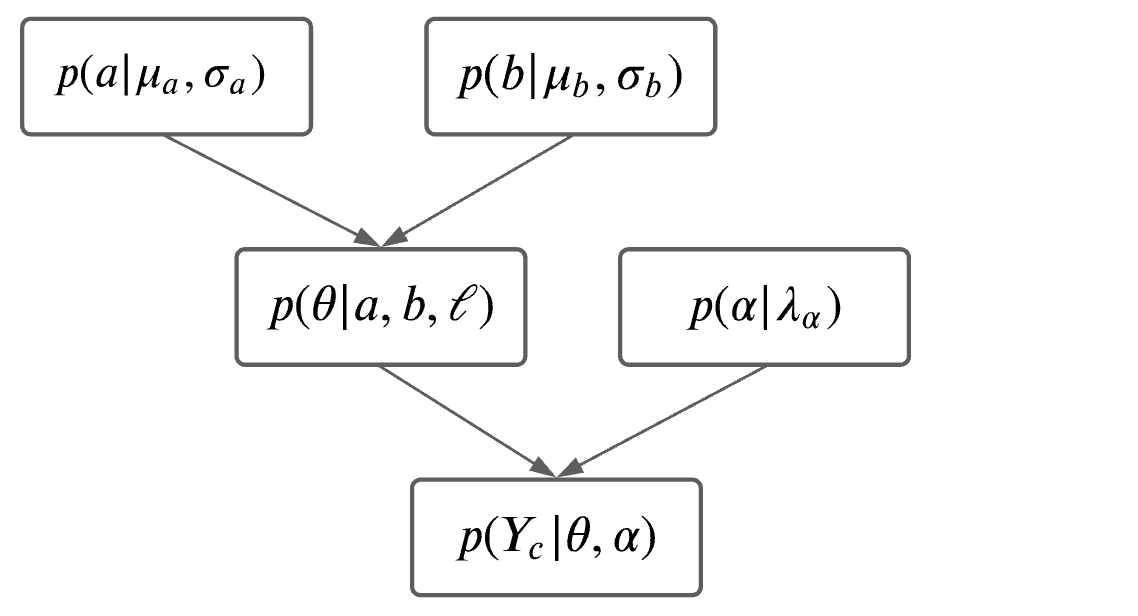
\includegraphics[width=10cm]{static/images/bayesian-network.png}
  \end{center}
  \caption{Bayesian network of incidence model}
  \label{fig:inc-model-bayesian-network}
\end{figure}

This definitely would not have an easy analytical solution, as we have to integrate over the domains of $\theta$, $\alpha$, $a$ and $b$ to obtain normalization constant, so lets employ MCMC theory through PyMC3 computation to help us to infer $X$.


\section{The inference of incidence}
\label{sec:inference-of-incidence}

We are now getting to the core of the problem itself, the inference of unknown parameters $X$ via PyMC3. 
Naturally, PyMC3 has to build its own internal representation of a model.
The internal representation looks like a \textit{directed acyclic graph} (DAG), which is very similar a Bayesian network in the figure \ref{fig:inc-model-bayesian-network}:

\begin{figure}[H]
  \begin{center}
    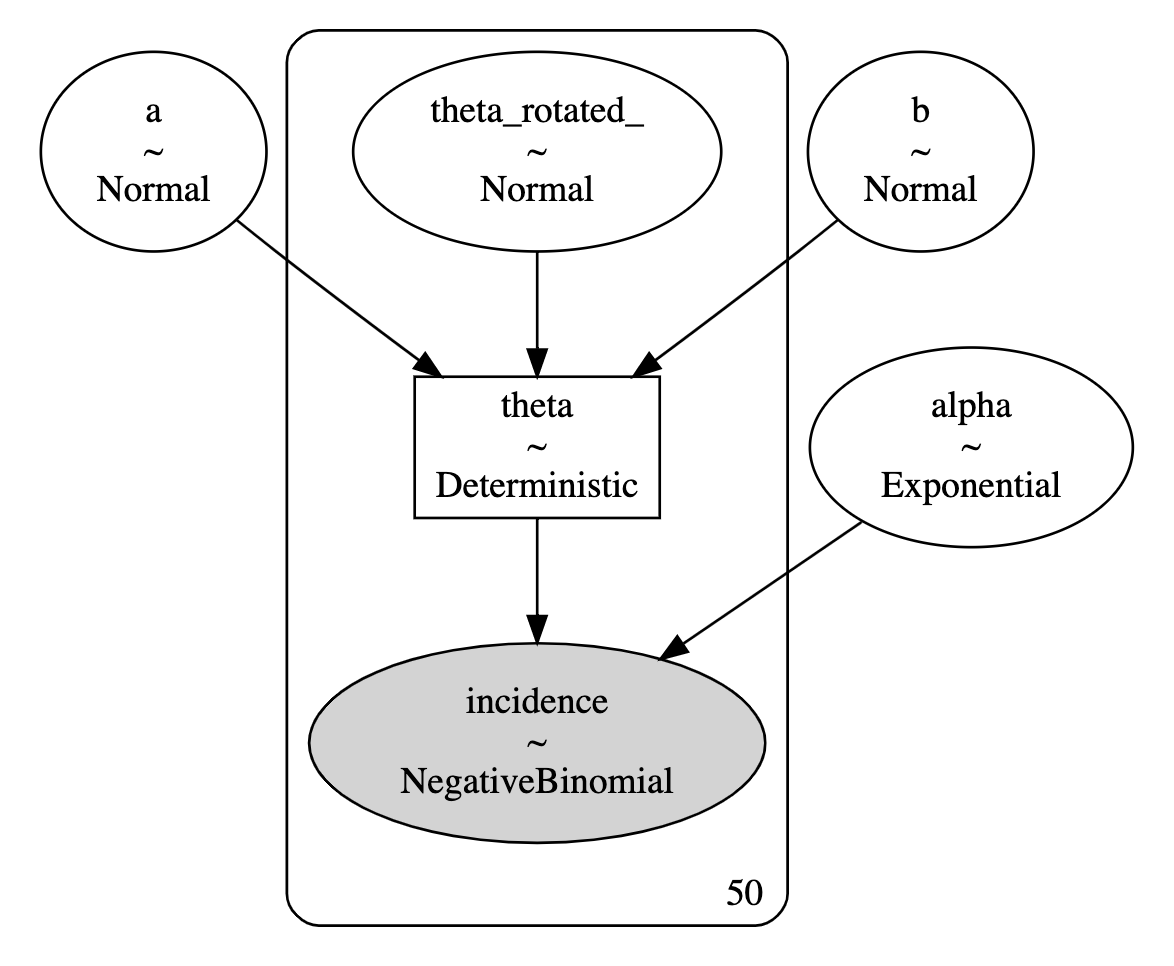
\includegraphics[width=8cm]{static/images/inc-model-graphviz.png}
  \end{center}
  \caption{Internal PyMC3 DAG representation of our incidence model}
  \label{fig:inc-model-graphviz}
\end{figure}

In the figure \ref{fig:inc-model-graphviz}\footnote{Created by Snippet \ref{snip:inc-model-graphviz}}, we can see how PyMC3 represents our particular incidence model (given by Snippet \ref{snip:inc-model-build-func}), where the shapes represents each particular distribution.
The highlighted shape is a likelihood, and the outlined shapes represent prior, similarly to our theoretical model \eqref{eq:inc-model-joint-expanded}.
The only minor discrepancy might be seen in PyMC3's representation of $\theta$.
This is given by the nature of $\theta$ as a Gaussian process, as it is basically multidimensional normal distribution, and PyMC3 uses\footnote{See \url{https://github.com/pymc-devs/pymc/blob/main/pymc/gp/gp.py\#L303}} rotating by \textit{Cholesky factor} \cite[Chapter 7]{murphy2021}.
In our case, the dimensionality of $\theta$ is equal to the size of the incidence window $T_w$.

To approximate incidence properly, we need to tune up the model for as many specific cases as possible. Ideally, we should try to approximate the whole incidence upon all the data; however, it would be very laborious due to the dimensionality of the data.

As was mentioned in Section \ref{sec:theta-analysis} we will estimate incidence for samples of size $T_w$ only instead of the whole time series.
In this particular case, as we have to tune the model, those samples should represent various heterogeneous cases to ensure the robustness of the model.
For this reason, we picked the following samples for incidence fitting:

\begin{enumerate}
  \item Noisy incidence as in the following figure\footnote{Created by Snippet \ref{snip:inc-model-sample-incidence-1}}:
  \begin{figure}[H]
    \begin{center}
      \includegraphics[width=9cm]{generated/images/inc-model-sample-incidence-1.png}
    \end{center}
    \caption{Sample 1 for the incidence inference tuning}
    \label{fig:dev-incidence-1}
  \end{figure}
  \item Zero-inflated incidence (Figure \ref{fig:dev-incidence-2}\footnote{Created by Snippet \ref{snip:inc-model-sample-incidence-2}})
  \item Regular growing incidence (Figure \ref{fig:dev-incidence-3}\footnote{Created by Snippet \ref{snip:inc-model-sample-incidence-3}})
\end{enumerate}


\subsection{Sampling}

For sampling the posterior distribution, we use NUTS, mentioned in Subsection \ref{sec:nuts}, because of its good performance in multidimensional problems.
In PyMC3, the NUTS sampler has several options to tune for better performance\footnote{See official documentation \url{https://docs.pymc.io/en/v3/api/inference.html}}, but for our case, the basic settings are sufficient.

Now we are ready for sampling.
Usually, in MCMC inference, we run several independent Markov chains in parallel.
This is because sometimes the convergence may not be successful, and it is not easily recognizable in the case of a single chain.

After sampling 4 chains, we obtain the following posterior distribution of $X$:

\begin{figure}[H]
  \begin{center}
    \includegraphics[width=13cm]{generated/images/inc-model-params-trace-1.png}
  \end{center}
  \caption{Posterior trace of parameters $X$ for sample 1}
  \label{fig:params-trace-1}
\end{figure}

On the left side, in the Figure \ref{fig:params-trace-1}\footnote{Created by Snippet \ref{snip:inc-model-sampling-trace-plot-1}}, we see results for each of the parameters $\theta$, $\alpha$, $a$ and $b$ as rows.
On the left side of the figure, we see how each particular chain for each variable performed in comparison with other chains of that variable.
On the right side, we see the chain of 500 samples we desired (samples from the burnin period are discarded) for each variable.
Note that the dimensionality of $\theta$ makes this figure slightly unclear.
For this purposes, we can plot the posterior of the Gaussian process in a separated plot\footnote{Created by Snippet \ref{snip:inc-model-theta-posterior-1}}:

\begin{figure}[H]
  \begin{center}
    \includegraphics[width=10cm]{generated/images/inc-model-theta-posterior-1.png}
  \end{center}
  \caption{Posterior of $\theta$ for sample 1}
  \label{fig:theta-posterior-1}
\end{figure}

The Figure \ref{fig:theta-posterior-1} may somehow remind the original data (actually, it should be the logarithm of the incidence mean).
To check if our model performed well, we usually need to plot something we can compare with some information we already know.
In the case of Bayesian inference, we can use \textit{posterior predictive check}.


\section{Posterior predictive check}

\textit{Posterior predictive check} (PPC) can be characterized as a replication of the original dataset from the inferred data. 
Basically, we reverse the inference algorithm, i.e., take inferred parameters and utilize them to generate an approximation of the observed data \cite{davidson-pilon2015}.
This allows us to see discrepancies between that approximation and observed data.

The following plots present the capability of fitting the observed incidence by the incidence model presented before.
The first plot is valid for the first sample (\ref{fig:dev-incidence-1}) of incidence observations defined in Section \ref{sec:inference-of-incidence}.

\newpage
To recall, the first sample represents noisy observations; PPC\footnote{Created by snippet \ref{snip:inc-model-ppc-plot-1}} of that sample looks like this:

\begin{figure}[H]
  \centering
  \includegraphics[width=11cm]{generated/images/inc-model-ppc-plot-1.png}
  \caption{Posterior predictive of $\hat{c}$ for sample 1}
  \label{fig:incidence-posterior-1}
\end{figure}

The second sample (Figure \ref{fig:dev-incidence-2}) represents zero-inflated incidence; PPC in the following figure\footnote{Created by Snippet \ref{snip:inc-model-ppc-plot-2}}:

\begin{figure}[H]
  \centering
  \includegraphics[width=10cm]{generated/images/inc-model-ppc-plot-2.png}
  \caption{Posterior predictive of $\hat{c}$ for sample 2}
  \label{fig:incidence-posterior-2}
\end{figure}

\newpage
And finally, the third sample (Figure \ref{fig:dev-incidence-3}) is for regularly growing incidence; PPC\footnote{Created by Snippet \ref{snip:inc-model-ppc-plot-3}}:

\begin{figure}[H]
  \centering
  \includegraphics[width=10cm]{generated/images/inc-model-ppc-plot-3.png}
  \caption{Posterior predictive of $\hat{c}$ for sample 3}
  \label{fig:incidence-posterior-3}
\end{figure}


\chapter{The risk estimation}

In the previous chapter, we achieved a proper settings to estimate incidence $\hat{c}$ via \textit{smoothening} of the observated noisy incidence $Y_c$.
Now we have to employ previously established epidemiological theory and utilize inferred incidence $\hat{c}$ to compute the risk.
To this end, we need to estimate prevalence $\hat{I}$, which we will approximate from $\hat{c}$.
The necessary theory was established in Chapter \ref{chap:epidemiological-prerequisites} and Section \ref{sec:data-based-approach}.

To be sure our solution works well, we need to validate the output values somehow. However, we do not know true prevalence because it is not available in the data we use.
Therefore, we will choose another approach.


\section{Synthetic dataset}

We will generate synthetic data from an artificial model with known parameters.
This artificial model should take effective reproduction number $\mathcal{R}_e$, which is the average number of infections caused by one infectee, as a parameter as we want to generate $\mathcal{R}_e$ on our own.
Moreover, this model should also produce $I$ to compare.
We will use the SIR model as the artificial model to generate data because of its extensive parameterization options. Unfortunately, the SIR model does not directly accept $\mathcal{R}_e$ parameter; therefore, we have to modify it.

Lets take equation \eqref{eq:sir-model-incidence} and discretize it by the Euler's method:

\begin{equation}
  \label{eq:risk-model-incidence}
  c = \beta_t I_{t-1} \frac{S_{t-1}}{N}
\end{equation}

Also discretize the equation \eqref{eq:sir-effective-reproduction-number} for $\mathcal{R}_e(t)$ for SIR model:

\begin{equation}\label{eq:risk-model-rt}
  \mathcal{R}_{et} = \mathcal{R}_0 \frac{S_{t-1}}{N} = \frac{\beta}{\gamma} \frac{S_{t-1}}{N}
\end{equation}

To incorporate $\mathcal{R}_{et}$ we will assume $\beta$ changes with time, hence $\beta_t$:

\begin{equation}
\beta_t = \frac{\gamma_t N \mathcal{R}_{et}}{S_{t-1}}
\end{equation}

The only thing that remains is to solve $\gamma$. According to \cite{ma2019}, the average mean time of infection can be assumed $\gamma^{-1}$.
For simplicity, we will use the expected value of serial interval $\omega$ as we are using its cumulative probability for incidence to prevalence transformation:

\begin{equation}
  \gamma = \frac{1}{\mathbb{E}[\omega]}
\end{equation}

\noindent
Substituting into incidence equation \eqref{eq:risk-model-incidence} we get:

\begin{equation}
  c = \gamma \mathcal{R}_{et} I_{t-1} = \frac{\mathcal{R}_{et} I_{t-1}}{\mathbb{E}[\omega]}
\end{equation}

\noindent
In our case, we artificially generate $\mathcal{R}_{e}$ via this function:

\begin{equation}
  \mathcal{R}_{e}(t) = 1 + \sin (0.03 * t) * \sin (0.05 * t)
\end{equation}

Assuming first 75 days, $\mathcal{R}_{e}(t)$ looks as follows:

\begin{figure}[H]
  \begin{center}
    \includegraphics[width=10cm]{generated/images/risk-model-fake-rt.png}
  \end{center}
  \caption{Generated $\mathcal{R}_{e}$}
  \label{fig:risk-model-fake-rt}
\end{figure}

With assumed parameters $N = 10000$, $I = 6$, $S = N - 1$, $R = 0$, the generated data are presented in the following figure:

\begin{figure}[H]
  \begin{center}
    \includegraphics[width=10cm]{generated/images/risk-model-fake-sir.png}
  \end{center}
  \caption{Generated SIR data}
  \label{fig:risk-model-fake-sir}
\end{figure}

The Figure \ref{fig:risk-model-fake-sir}\footnote{Created by Snippet \ref{snip:risk-model-fake-sir-plot}} represents the SIR curves for the artifical model, but this will be utilized rather later.
More essential now is the incidence, as we first need to estimate it as we established in the previous chapter.
To not make it easy for our incidence model, we will simulate the seasonality from the original data with harmonic oscillation defined as:

\begin{equation}
  h(t) = A \cos(\psi t + \varphi),
\end{equation}

where $A$ is amplitude, $\psi$ is angular frequency and $\varphi$ is shift.
We will assume observation as a product of the true value of $c$
and the oscillator:

\begin{equation}
  Y_{c}(t) = c(t) h(t)
\end{equation}

Now we need to adjust our oscillation function.
The original function oscilates around 0, so we have to shift it by 1 to get values between 0.5 and 1.5.
Next, let apply weekly periodicity $\psi = \frac{2 \pi}{T} = \frac{2 \pi}{7}$, and $\varphi = \frac{\pi}{2}$ to have $h_{adj}(0) = 1$:

\begin{equation}
  h_{adj}(t) = 1 + cos \left( \frac{2 \pi}{7} t + \frac{\pi}{2} \right)
\end{equation}

Employing the previous, the observation generation equation has currently this form:

\begin{equation}
  Y_{c}(t) = c(t) h_{adj}(t)
\end{equation}

The plot of true and observed incidence, $Y_{c}$ and $c$ respectively, from the equation above, is the following:

\begin{figure}[H]
  \begin{center}
    \includegraphics[width=10cm]{generated/images/risk-model-fake-incidence.png}
  \end{center}
  \caption{Generated true and observed incidence}
  \label{fig:risk-model-fake-incidence}
\end{figure}

If we fit the observed data, we obtain the plot in Figure \ref{fig:risk-model-incidence-posterior-predictive}\footnote{Created by snippet \ref{snip:risk-model-fake-inc-posterior}} suggesting a good fit in terms of noisiness in the observed data.

\begin{figure}[H]
  \begin{center}
    \includegraphics[width=10cm]{generated/images/risk-model-incidence-posterior-predictive.png}
  \end{center}
  \caption{Posterior plot of $\hat{c}$, also with true and observed incidence}
  \label{fig:risk-model-incidence-posterior-predictive}
\end{figure}


\section{Prevalence estimation}

To proceed to the prevalence estimation $\hat{I}$, we can discretize the equation \eqref{eq:prevalence-int} to:

\begin{equation}\label{eq:prevalence-sum}
  I_t = \sum_{a=0}^{a_{max}} c_{t - a} \bar{\Omega}_a
\end{equation}

to recall, $a$ is infectious age and $\Omega$ is a cumulative distribution function of serial interval, which is computed from equation \eqref{eq:Omega-int}, which can be discretized in this fashion:

\begin{equation}
  \bar{\Omega}_a = 1 - \sum_{j = 1}^a \omega_j
\end{equation}

\noindent
where $\omega_j$ is a particular value of serial interval such that $\sum_{j = 1}^{a_{max}} \omega_j = 1$.

After swaping the variables for estimations, we obtain\footnote{See snippet \ref{snip:risk-model-prevalence-matrix}}:

\begin{equation}\label{eq:prevalence-est}
  \hat{I}_t = \sum_{a=0}^{a_{max}} \hat{c}_{t - a} \bar{\Omega}_a
\end{equation}

And the plot of $\hat{I}_t$ in this synthetic-data case is shown in figure \ref{fig:risk-model-prevalence-est}\footnote{Created by snippet \ref{snip:risk-model-prevalence-plot}}.
There is also the original $I$ for comparison, how well we did the estimation.

\begin{figure}[H]
  \begin{center}
    \includegraphics[width=12cm]{generated/images/risk-model-prevalence-est.png}
  \end{center}
  \caption{Estimation of prevalence}
  \label{fig:risk-model-prevalence-est}
\end{figure}

We can see quite well fit with minor discrepancy caused obviously by the small underestimation in the incidence, as we may see in the posterior plot in the Figure \ref{fig:risk-model-incidence-posterior-predictive}.


\section{Reproduction number estimation}

As we have $\hat{c}$ and $\omega$ available, we can easily use the Fraser model (mentioned in Section \ref{sec:fraser-model}) to make estimation $\hat{\mathcal{R}}_{et}$ of effective reproduction number $\mathcal{R}_e$.
This is not a necessary step in the way to estimate the risk, but it is a very good step for validation as the Fraser model does not rely on previously computed prevalence $\hat{I}$ but only incidence $\hat{c}$.

After discretization of the equation \eqref{eq:fraser-Re}, we obtain equation for the estimation $\hat{\mathcal{R}}_{et}$:

\begin{equation}
  \hat{\mathcal{R}}_{et} = \frac{\hat{c}_t}{\sum_a^{a_{max}} \hat{c}_{t - a} \omega_a}
\end{equation}

The previous is visualized in the following plot\footnote{Created by snippet \ref{snip:risk-model-reproduction-figure}}, again, with the true $\mathcal{R}_e$:

\begin{figure}[H]
  \begin{center}
    \includegraphics[width=12cm]{generated/images/risk-model-reproduction-est.png}
  \end{center}
  \caption{Estimation of effective reproduction number $\mathcal{R}_e$}
  \label{fig:risk-model-reproduction-est}
\end{figure}

Again, the estimation performs well.
The true reproduction number $\mathcal{R}_e$ is not exceeding the $95 \%$ of the confidence interval.


\section{Risk computation}

In the Chapter \ref{chap:risk-as-probability}, we introduced hypergeometric distribution to express the risk.
There, $N$, $I$, $n$, and $i$ were assumed as population size, prevalence, number of contacts (sample size), and number of infectious contacts, respectively.
Instead of $I$, we can employ our estimation $\hat{I}_t$ and place it into the equation \eqref{eq:risk-theoretic}:


\begin{equation}
  P_t(i \geq 1|n) = 1 - \frac{
    \binom{N - \hat{I}_t}{n}
  }{
    \binom{N}{n}
  }
\end{equation}

Applying this equation to the estimated prevalence, we obtain the following time series of infection probabilities\footnote{Created by Snippet \ref{snip:risk-model-risk-est-plot}}:

\begin{figure}[H]
  \begin{center}
    \includegraphics[width=12cm]{generated/images/risk-model-risk-est.png}
  \end{center}
  \caption{Estimation of probability of infectious contact}
  \label{fig:risk-model-risk-est}
\end{figure}


\section{The real data based example}

In the previous section, the risk model showed it could perform well on the synthetic dataset.
Now is the time to test our model in real conditions.
For this purpose, we will utilize the data we described previously.
Let estimate the risk for the whole South Moravian region (7 districts), which is summarized in the following table:

\input{generated/tables/real-data-risks.tex}

According to this table, $\sum_u \mathbb{E}[\hat{I}^{(u)}] = 8 133$ and $\sum_u I_\text{naive}^{(u)} = 34 878$, where $u$ is each district in the South Moravian region, and $I_\text{naive}$ is the prevalence computed by the naive method from the equation \eqref{eq:data-prevalence-naive}, i.e., $I_\text{naive}^{(u)} = Y_C^{(u)} - Y_R^{(u)} - Y_D^{(u)}$ (Figure \ref{fig:real-data-prevalence}).

For the South Moravian region, there is a page\footnote{\url{https://onemocneni-aktualne.mzcr.cz/covid-19/kraje/JHM}} at the official Covid-19 portal, where \textit{number of active cases} is \textit{33 553} (to the same date) which is much closer to the $\sum_u I_\text{naive}^{(u)}$ than our estimation $\sum_u \mathbb{E}[\hat{I}^{(u)}]$.
As we assume the estimation from the official authorities to be the source of truth, our model does not give the proper results.
The model substantially underestimates the prevalence.
This means the real risk might be much higher than the risk shown in table \ref{tab:real-data-risks}.

Unfortunately, the proper description of how the official authorities approach the prevalence could not be found to compare or calibrate the model. Moreover, our model does not take undetected cases into account, which really matters in reality \cite{simone2020}.


\chapter{Conclusion}

In the beginning, we presented minimal epidemiological theory needed to understand the approach in this thesis; then the real-world situation was presented.
First, the data was gathered and analyzed to know its form.
Then the model, consisting of two parts, was built upon.
The first part is the probabilistic incidence approximation, which is then utilized in the second part - the risk computation, which is deterministic in its nature, but, as it is built upon the posterior predictive of incidence, it provides uncertainty intervals to compute the final risk of infectious contact.

This thesis should be understood as exploring the intricacies in probabilistic modelling rather than providing an accurate tool.
The hope is that the lessons learned and presented as a part of this thesis will help the reader build their own, potentially more precise epidemiological solution.

Please consider this as an example of how probabilistic programming can be used in epidemiological modelling, as this solution is not accurate on real data yet.


\printbibliography[heading=bibintoc]

\appendix

\chapter{Additional tables}


\input{generated/tables/data-adf-test-brno}
\input{generated/tables/data-adf-test-ostrava}


\chapter{Additional figures}

\begin{figure}[H]
  \begin{center}
    \includegraphics[width=\textwidth]{generated/images/inc-model-sample-incidence-2.png}
  \end{center}
  \caption{Sample 2 - zero-inflated}
  \label{fig:dev-incidence-2}
\end{figure}

\begin{figure}[H]
  \begin{center}
    \includegraphics[width=\textwidth]{generated/images/inc-model-sample-incidence-3.png}
  \end{center}
  \caption{Sample 3 - regular growth}
  \label{fig:dev-incidence-3}
\end{figure}



\begin{figure}[H]
  \begin{center}
    \includegraphics[width=11cm]{generated/images/inc-model-params-trace-2.png}
  \end{center}
  \caption{Posterior trace of parameters $X$ for sample 2}
  \label{fig:params-trace-2}
\end{figure}



\begin{figure}[H]
  \begin{center}
    \includegraphics[width=11cm]{generated/images/inc-model-params-trace-3.png}
  \end{center}
  \caption{Posterior trace of parameters $X$ for sample 3}
  \label{fig:params-trace-3}
\end{figure}




\begin{figure}[H]
  \begin{center}
    \includegraphics[width=\textwidth]{generated/images/inc-model-theta-posterior-2.png}
  \end{center}
  \caption{Posterior of $\theta$ for sample 2}
  \label{fig:theta-posterior-2}
\end{figure}

\begin{figure}[H]
  \begin{center}
    \includegraphics[width=\textwidth]{generated/images/inc-model-theta-posterior-3.png}
  \end{center}
  \caption{Posterior of $\theta$ for sample 3}
  \label{fig:theta-posterior-3}
\end{figure}

\newpage
This is how the posterior distribution for the sample from figure \ref{fig:dev-incidence-1} will look when we use zero mean in the Gaussian process:

\begin{figure}[H]
  \centering
  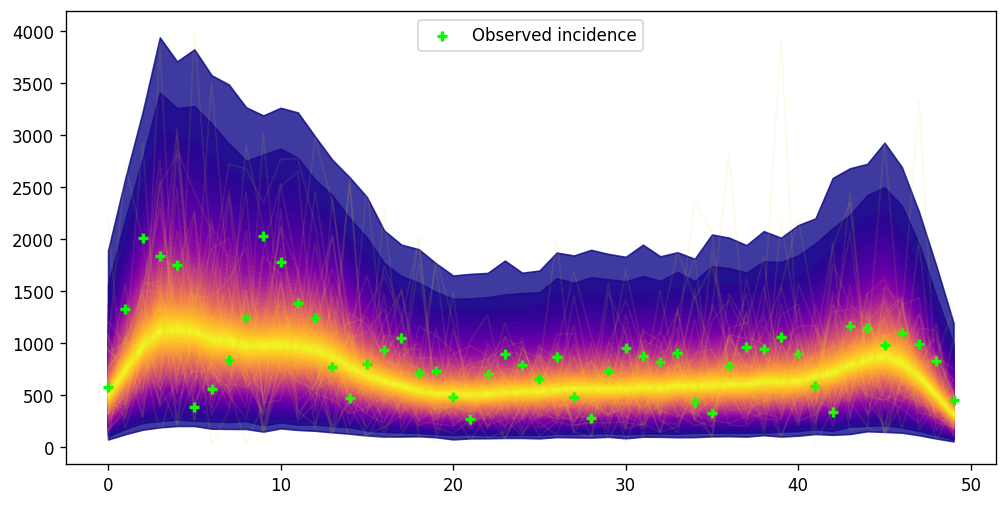
\includegraphics[width=11cm]{static/images/inc-model-ppc-plot-1-zero-mean.png}
  \caption{Posterior predictive of $\hat{c}$ for sample 1 with zero mean GP}
  \label{fig:incidence-posterior-1-zero-mean}
\end{figure}



\begin{figure}[H]
  \begin{center}
    \includegraphics[width=11cm]{generated/images/real-data-prevalence.png}
  \end{center}
  \caption{Prevalence computed via naive approach from the raw data}
  \label{fig:real-data-prevalence}
\end{figure}



\chapter{The code snippets}

Most of the Jupyter notebook cells are available in the following snippets, which were continuously referenced in the thesis.
Those should help understand the chosen approach if the text is insufficient for a reader.
We do not recommend using those cells to replicate the notebook, as some were deflated to save space.
To do experiments, use rather the full notebook available here \url{https://github.com/sheater/fimscthesis/blob/master/main.ipynb}.


\section{Notebook initialization}

\input{generated/snippets/init-installs.tex}
\input{generated/snippets/init-imports.tex}

\section{Utilities}

\input{generated/snippets/config.tex}

\input{generated/snippets/utils-base-figure.tex}
\input{generated/snippets/utils-base-plotly.tex}
\input{generated/snippets/utils-base-matplotlib.tex}
\input{generated/snippets/utils-base-latex.tex}
\input{generated/snippets/utils-data-node.tex}
\input{generated/snippets/hyperparameters.tex}
% \input{generated/snippets/utils-cz-root.tex}
\input{generated/snippets/utils-adf-test}

\section{Data wrangling}

\input{generated/snippets/data-serial-interval-base.tex}
\input{generated/snippets/data-serial-interval-instances.tex}
\input{generated/snippets/data-serial-intervals-overview.tex}
\input{generated/snippets/data-serial-intervals-Omega.tex}
\input{generated/snippets/data-incidence.tex}
\input{generated/snippets/data-node-instances.tex}
\input{generated/snippets/data-largest-cities-plot.tex}
\input{generated/snippets/data-adf-test-prague.tex}
\input{generated/snippets/data-adf-test-brno-ostrava.tex}
\input{generated/snippets/data-seasonal-decomposition-figure.tex}
\input{generated/snippets/data-seasonal-decomposition-additive.tex}
\input{generated/snippets/data-seasonal-decomposition-multiplicative.tex}

\section{Incidence model}

\input{generated/snippets/incidence-log-transform-plot.tex}
\input{generated/snippets/theta-diff-plot.tex}
\input{generated/snippets/theta-diff-sample-windows-plot.tex}
\input{generated/snippets/theta-diff-histogram.tex}
\input{generated/snippets/theta-diff-qq-plot.tex}
\input{generated/snippets/theta-diff-ecdf-plot.tex}
% FIXME:
\input{generated/snippets/theta-diff-ks-test.tex}
\input{generated/snippets/theta-diff-lilliefors-test.tex}
\input{generated/snippets/theta-diff-shapiro-wilk-test.tex}

\input{generated/snippets/inc-model-sample-incidence-figure.tex}
\input{generated/snippets/inc-model-sample-incidence-1.tex}
\input{generated/snippets/inc-model-sample-incidence-2.tex}
\input{generated/snippets/inc-model-sample-incidence-3.tex}

\input{generated/snippets/inc-model-build-func.tex}
\input{generated/snippets/inc-model-build-on-samples.tex}
\input{generated/snippets/inc-model-graphviz.tex}
\input{generated/snippets/inc-model-sampling-func.tex}
\input{generated/snippets/inc-model-sampling-1.tex}
\input{generated/snippets/inc-model-sampling-2.tex}
\input{generated/snippets/inc-model-sampling-3.tex}
\input{generated/snippets/inc-model-trace-figure.tex}
\input{generated/snippets/inc-model-sampling-trace-plot-1.tex}
\input{generated/snippets/inc-model-sampling-trace-plot-2.tex}
\input{generated/snippets/inc-model-sampling-trace-plot-3.tex}
\input{generated/snippets/inc-model-theta-posterior-figure.tex}
\input{generated/snippets/inc-model-theta-posterior-1.tex}
\input{generated/snippets/inc-model-theta-posterior-2.tex}
\input{generated/snippets/inc-model-theta-posterior-3.tex}

\input{generated/snippets/inc-model-pp-func.tex}
\input{generated/snippets/inc-model-ppc-1.tex}
\input{generated/snippets/inc-model-ppc-2.tex}
\input{generated/snippets/inc-model-ppc-3.tex}
\input{generated/snippets/inc-model-ppc-figure.tex}
\input{generated/snippets/inc-model-ppc-plot-1.tex}
\input{generated/snippets/inc-model-ppc-plot-2.tex}
\input{generated/snippets/inc-model-ppc-plot-3.tex}

\section{Risk model}

\input{generated/snippets/risk-model-fake-rt.tex}
\input{generated/snippets/risk-model-fake-sir.tex}
\input{generated/snippets/risk-model-fake-sir-plot.tex}
\input{generated/snippets/risk-model-fake-incidence.tex}
\input{generated/snippets/risk-model-fake-inference.tex}
\input{generated/snippets/risk-model-fake-inc-posterior.tex}
\input{generated/snippets/risk-model-prevalence-matrix.tex}
\input{generated/snippets/risk-model-helper-quantile-traces.tex}
\input{generated/snippets/risk-model-prevalence-plot.tex}
\input{generated/snippets/risk-model-reproduction-matrix.tex}
\input{generated/snippets/risk-model-reproduction-figure.tex}
\input{generated/snippets/risk-model-risk-est-plot.tex}


\section{The real data based example}

\input{generated/snippets/examples-incidence-estimate-func.tex}
\input{generated/snippets/examples-southbohemian-region-inference.tex}
\input{generated/snippets/examples-southbohemian-region-table.tex}
\input{generated/snippets/examples-southbohemian-region-crude.tex}


\end{document}
